   %% LyX 2.3.4.2 created this file.  For more info, see http://www.lyx.org/.
%% Do not edit unless you really know what you are doing.
\documentclass[12pt,oneside,american,czech]{book}
\usepackage[T1]{fontenc}
\usepackage[utf8]{inputenc}
\usepackage[a4paper]{geometry}
\geometry{verbose,tmargin=4cm,bmargin=3cm,lmargin=3cm,rmargin=2cm,headheight=0.8cm,headsep=1cm,footskip=0.5cm}
\pagestyle{headings}
\setcounter{secnumdepth}{3}
\usepackage{url}
\usepackage{amsmath}
\usepackage{amsthm}
\usepackage{amssymb}
\usepackage{graphicx}
\usepackage{setspace}
\usepackage{hyperref}
\usepackage{libertine}
\usepackage{comment}
\usepackage{calrsfs}
\usepackage{subfig}
\makeatletter
%%%%%%%%%%%%%%%%%%%%%%%%%%%%%% Textclass specific LaTeX commands.
\newenvironment{lyxlist}[1]
	{\begin{list}{}
		{\settowidth{\labelwidth}{#1}
		 \setlength{\leftmargin}{\labelwidth}
		 \addtolength{\leftmargin}{\labelsep}
		 \renewcommand{\makelabel}[1]{##1\hfil}}}
	{\end{list}}

%%%%%%%%%%%%%%%%%%%%%%%%%%%%%% User specified LaTeX commands.
%% Font setup: please leave the LyX font settings all set to 'default'
%% if you want to use any of these packages:

%% Use Times New Roman font for text and Belleek font for math
%% Please make sure that the 'esint' package is turned off in the
%% 'Math options' page.
\usepackage[varg]{txfonts}

%% Use Utopia text with Fourier-GUTenberg math
%\usepackage{fourier}

%% Bitstream Charter text with Math Design math
%\usepackage[charter]{mathdesign}

%%---------------------------------------------------------------------

%% Make the multiline figure/table captions indent so that the second
%% line "hangs" right below the first one.
%\usepackage[format=hang]{caption}

%% Indent even the first paragraph in each section
\usepackage{indentfirst}

%%---------------------------------------------------------------------

%% Disable page numbers in the TOC. LOF, LOT (TOC automatically
%% adds \thispagestyle{chapter} if not overriden
%\addtocontents{toc}{\protect\thispagestyle{empty}}
%\addtocontents{lof}{\protect\thispagestyle{empty}}
%\addtocontents{lot}{\protect\thispagestyle{empty}}

%% Shifts the top line of the TOC (not the title) 1cm upwards 
%% so that the whole TOC fits on 1 page. Additional page size
%% adjustment is performed at the point where the TOC
%% is inserted.
%\addtocontents{toc}{\protect\vspace{-1cm}}

%%---------------------------------------------------------------------

% completely avoid orphans (first lines of a new paragraph on the bottom of a page)
\clubpenalty=9500

% completely avoid widows (last lines of paragraph on a new page)
\widowpenalty=9500

% disable hyphenation of acronyms
\hyphenation{CDFA HARDI HiPPIES IKEM InterTrack MEGIDDO MIMD MPFA DICOM ASCLEPIOS MedInria}

%%---------------------------------------------------------------------

%% Print out all vectors in bold type instead of printing an arrow above them
\renewcommand{\vec}[1]{\boldsymbol{#1}}
\newcommand{\R}{\mathbb{R}}
\newtheorem{theorem}{Věta}[section]
\newtheorem*{poz}{Poznámka}
\theoremstyle{definition}
\newtheorem{definition}{Definice}[section]

\newtheorem{vet}{Věta}[section]

\newtheorem*{pří}{Příklad}
\newcommand{\N}{\mathbb{N}}
\newcommand{\C}{\mathbb{C}}
\newcommand{\Z}{\mathbb{Z}}
%  Matematika
\newcommand{\ee}{\mathrm{e}} %eulerovo číslo
\newcommand{\ii}{\mathrm{i}} %imaginární jednotka
\newcommand{\inR}{\in \mathbb{R}}
\newcommand{\dd}{\mathrm{d}}
\newcommand\KLDeq{\mathrel{\stackrel{\makebox[0pt]{\mbox{\normalfont\tiny KLD}}}{\approx}}}
\newcommand*{\matr}[1]{\mathbfit{#1}}
\newcommand*{\tran}{^{\mkern-1.5mu\mathsf{T}}}
\newcommand*{\conj}[1]{\overline{#1}}
\newcommand*{\hermconj}{^{\mathsf{H}}}
\DeclareMathOperator{\tr}{tr}
\DeclareMathOperator*{\argmin}{arg\,min} 
\DeclareMathOperator*{\argmax}{arg\,max} 
\DeclareMathAlphabet{\pazocal}{OMS}{zplm}{m}{n}
% Jednotky
\newcommand{\unit}[1]{\,\mathrm{#1}} %jednotky zadávejte pomocí tohoto příkazu
\renewcommand{\deg}{\ensuremath{\mathring{\;}}} %symbol stupně
\newcommand{\celsius}{\ensuremath{\deg\mathrm{C}}} %stupně celsia

%(hodnota plus mínus chyba) jednotka
\newcommand{\hodn}[3]{(#1 \pm #2)\unit{#3}} 

%veličina [jednotka] do hlavičky tabulky
\newcommand{\tabh}[2]{\ensuremath{#1\,[\mathrm{#2}]}} 
% Replace standard \cite by the parenthetical variant \citep
%\renewcommand{\cite}{\citep}
\newcommand{\diag}{\mathop{\mathrm{diag}}}
\def\Var{{\textrm{Var}}\,}



\makeatother

\usepackage{babel}
\begin{document}
\def\documentdate{7. \v{c}ervence 2020}

%%\def\documentdate{\today}

\pagestyle{empty}
{\centering

\noindent %
\begin{minipage}[c]{3cm}%
\noindent \begin{center}

\includegraphics[width=3cm,height=3cm,keepaspectratio]{Images/TITLE/cvut}
\par\end{center}%
\end{minipage}%
\begin{minipage}[c]{0.6\linewidth}%
\begin{center}
\textsc{\large{}České vysoké učení technické v Praze}{\large{}}\\
{\large{}Fakulta jaderná a fyzikálně inženýrská}
\par\end{center}%
\end{minipage}%
\begin{minipage}[c]{3cm}%
\noindent \begin{center}

\includegraphics[width=3cm,height=3cm,keepaspectratio]{Images/TITLE/fjfi}
\par\end{center}%
\end{minipage}

\vspace{3cm}

\textbf{\huge{Generativní modely dat popsaných stromovou strukturou}}{\huge\par}

\vspace{1cm}

\selectlanguage{american}%
\textbf{\huge{Generative models of tree structured data}}{\huge\par}

\selectlanguage{czech}%
\vspace{2cm}

{\large{}Bakalářská práce}{\large\par}

}

\vfill{}

\begin{lyxlist}{MMMMMMMMM}
\begin{singlespace}
\item [{Autor:}] \textbf{Jakub Bureš}
\item [{Vedoucí~práce:}] \textbf{Doc. Ing. Václav Šmídl, Ph.D.}
\item [{Konzultant:}] \textbf{Doc. Ing. Tomáš Pevný, Ph.D.}
\item [{Akademický~rok:}] 2019/2020
\end{singlespace}
\end{lyxlist}
\newpage{}

~

\vfill{}

\begin{center}
\begin{enumerate}	
\item Seznamte se s popisem dat pomocí stromové struktury. Zvláštní pozornost věnujte metodám více instančního učení (multiple instance learning). Seznamte se s konceptem vnořeného prostoru (embedded space) a jeho reprezentace pomocí neuronových sítí. 
\item	
Seznamte se se základními generativními modely dat popsaných vektorem příznaků. Zvláštní pozornost věnujte metodám typu autoencoder a jejich variační formě. Demonstrujte vlastnosti modelů na jednoduchých příkladech. V maximální míře využijte dostupné knihovny pro generativní modely.
\item
Navrhněte několik příkladů typů dat se stromovou strukturou a pro každý z nich navrhněte generativní model. Navrhněte algoritmus pro určení jeho parametrů z dat a diskutujte vhodnost jednotlivých architektur neuronových sítí.
\item
Seznamte se s různými druhy apriorních rozložení používaných na latentní proměnné autoencoderu. Odvoďte algoritmy odhadu jejich parametrů a srovnejte jejich výsledky se základním modelem. Diskutujte výsledné odhady.
\item	
Vyvinutou metodu aplikujte na vhodně zvolená reálná data a diskutujte vliv zvoleného apriorního rozložení na výsledky.
\end{enumerate}
\par\end{center}

\vfill{}

~\newpage{}

~

\vfill{}

\begin{center}
- Zadání práce (zadní strana) -
\par\end{center}

\vfill{}

~\newpage{}

\noindent \emph{\Large{}Poděkování:}{\Large\par}

\noindent Chtěl bych zde poděkovat především svému školiteli panu Doc. Ing. Václavu Šmídlovi, Ph.D.
za pečlivost, ochotu, vstřícnost a odborné i lidské zázemí při vedení
mé bakalářské práce. Dále děkuji svému konzultantovi panu Doc. Ing. Tomáši Pevnému, Ph.D.

\vfill

\noindent \emph{\Large{}Čestné prohlášení:}{\Large\par}

\noindent Prohlašuji, že jsem tuto práci vypracoval samostatně a uvedl
jsem všechnu použitou literaturu.

\bigskip{}

\noindent V Praze dne \documentdate\hfill{}Jakub Bureš

\vspace{2cm}

\newpage{}

\begin{onehalfspace}
\noindent \emph{Název práce:} 

\noindent \textbf{Generativní modely dat popsaných stromovou strukturou}
\end{onehalfspace}

\bigskip{}

\noindent \emph{Autor:} Jakub Bureš

\bigskip{}

\noindent \emph{Obor:} Matematické inženýrství
 \bigskip{}

\noindent \emph{Zaměření:} Aplikované matematicko-stochastické metody

\bigskip{}

\noindent \emph{Druh práce:} Bakalářská práce

\bigskip{}

\noindent \emph{Vedoucí práce:} Doc. Ing. Václav Šmídl, Ph.D.\\
ÚTIA AV ČR
Pod vodárenskou věží 4
182 00 Praha 8

\bigskip{}

\noindent \emph{Konzultant:} Doc. Ing. Tomáš Pevný, Ph.D. \\
Katedra počítačů
FEL ČVUT Praha
Technická 1902/2
166 27 Praha 6 - Dejvice
\bigskip{}

\noindent \emph{Abstrakt:} 
Tato bakalářská práce řeší 
\bigskip{}

\noindent \emph{Klíčová slova:} klíčová slova (nebo výrazy) seřazená
podle abecedy a oddělená čárkou

\vfill{}
~

\selectlanguage{american}%
\begin{onehalfspace}
\noindent \emph{Title:}Generative models of tree structured data 

\noindent \textbf{Generative models of tree structured data}
\end{onehalfspace}

\bigskip{}

\noindent \emph{Author:} Jakub Bureš

\bigskip{}

\noindent \emph{Abstract:} Max. 10 lines of English abstract text.
Max. 10 lines of English abstract text. Max. 10 lines of English abstract
text. Max. 10 lines of English abstract text. Max. 10 lines of English
abstract text. Max. 10 lines of English abstract text. Max. 10 lines
of English abstract text. Max. 10 lines of English abstract text.
Max. 10 lines of English abstract text. Max. 10 lines of English abstract
text. Max. 10 lines of English abstract text. Max. 10 lines of English
abstract text. Max. 10 lines of English abstract text. Max. 10 lines
of English abstract text. Max. 10 lines of English abstract text.
Max. 10 lines of English abstract text. Max. 10 lines of English abstract
text. Max. 10 lines of English abstract text. Max. 10 lines of English
abstract text. Max. 10 lines of English abstract text. Max. 10 lines
of English abstract text. Max. 10 lines of English abstract text.
Max. 10 lines of English abstract text. Max. 10 lines of English abstract
text. Max. 10 lines of English abstract text.

\bigskip{}

\noindent \emph{Key words:} keywords in alphabetical order separated
by commas

\selectlanguage{czech}%
\newpage{}

\pagestyle{plain}

\tableofcontents{}

\newpage{}




\chapter*{Úvod}
Internet se stal nedílnou součástí našich životů a mnozí si už ani nedokáží představit, jak by bez něho řešili každodenní starosti. Nakupujeme, prodáváme, spravujeme naše finance, píšeme zprávy a mnoho dalšího pomocí internetu. Zde vyvstává otázka internetové bezpečnosti. Je toto všechno bezpečné?  Se zvyšujícím se provozem v internetu, se zvyšuje též počet pokusů o jeho zneužití, ať už pomocí virů, odposlouchávání, botnetů či malwaru obecně. Tradiční obranná řešení se spoléhají na identifikaci předem stanovených znaků, kterými se malware liší od neškodného programu. Inteligence a adaptivita malwaru však neustále roste a prakticky tak znemožňuje nalezení deterministických pravidel či postupů k jeho detekci. \\
Cílem této bakalářské práce je nejprve seznámit se s postupy využívající strojové učení, které dokáží sestavit pravděpodobnostní model vhodný pro nalezení anomálií v síťovém provozu. To zahrnuje nezbytný matematický aparát, jmenovitě optimalizaci, pravděpodobnostní počet a statistiku, přičemž se předpokládá základní znalost diferenciálního a integrálního počtu Za druhé tato práce vysvětluje problematiku na jednoduchých příkladech. Měla by sloužit jako odrazový můstek, tudíž by na ní mělo být navázáno prací diplomovou, jejímž cílem by mělo být hledání konkrétního modelu aplikovatelného na reálná data.


\pagestyle{headings}
\chapter{Teorie}
\section{Optimalizace}
Optimalizace je matematická úloha, jejíž snahou je nalezení takových hodnot proměnných, pro které daná funkce nabývá minima či maxima. My se budeme snažit najít minimální hodnoty vektoru parametrů $\theta$ tzv. ztrátové funkce $\textit{(loss function)}$. Ztrátovou funkci budeme dle anglického výrazu značit $L(\theta)$. 
Minimalizací ztrátové funkce získáme odhad parametrů
\begin{equation}\label{argminL}
\hat{\theta} = \argmin_{\theta} L(\theta),
\end{equation}
který budeme vždy značit pomocí stříšky. Existuje nespočet způsobů jak danou funkci minimalizovat. My budeme výhradně používat metodu zvanou Gradient Descent. 

\subsection{Gradient Descent}
Jedná se o iterativní optimalizační metodu. 
  Minimalizujeme $L(\theta)$, tedy derivujeme dle vektoru parametrů $\theta$, díky čemuž dostaneme $\nabla_{\theta}\ L(\theta) $. Symbol $\nabla_{\theta}$ značí gradient funkce $L(\theta)$ přes všechny hodnoty $\theta$.
Použijeme bod $\theta_0$ funkce $L(\theta)$ jako výchozí bod. Jelikož gradient udává směr nejvyššího růstu pohybujeme se ve směru záporného gradientu a to s krokem $h$~$\in$~$\mathbb{R}_{+}$.  Matematickou interpretaci toho postupu můžeme vyjádřit následujícím zápisem
\begin{equation}\label{GradientDescent}
\theta_{n+1} = \theta_{n} - h\cdot \nabla_{\theta} L(\theta_n).
\end{equation}
 Tento postup provádíme, dokud nejsme v minimu funkce a získáme tak vektor parametrů $\hat{\theta}$, jak je popsáno v \eqref{argminL}. Ačkoliv se tento algoritmus může zdát na první pohled jako silný nástroj při řešení optimalizačních úloh, ve skutečnosti je opak pravdou. Ve velkých dimenzích a obrovském množství dat je tato metoda pomalá a prakticky se nepoužívá. 
\subsection*{ADAM}
Kvůli důvodům uvedeným výše, používáme vylepšenou gradientní metodu, tzv. adaptivní iterační metodu ADAM \textit{(Adaptive Moment Estimation)} [], která navíc používá druhý moment gradientu. Zatímco Gradient Descent má krok stále stejný, u metody ADAM je krok $h$ adaptivní. Více ji specifikovat v tomto textu nebudeme. Pro nás je důležité, že je tento algoritmus silnější a mnohem rychlejší v řešení složitých optimalizačních úloh. 

\subsection{Metoda nejmenších čtverců}\label{least_squares}
 Metoda nejmenších čtverců je nejzákladnější metoda pro hledání nejlepší proložení určitých dat nějakou křivkou. Představíme zjednodušenou alternativu, jak tuto metodu odvodit. Předpokládejme, že máme množinu $\textbf{x} = \left \lbrace x_{i}\right\rbrace_{i = 1}^{n} $, kde ke každému $x_i$ máme právě jedno pozorování $y_i$, které je zatíženo nějakou neznámou chybou $\varepsilon_i$. Označme $\mathbf{y} = \left\lbrace y_{i}\right\rbrace_{i = 1}^{n}$, komplexně zapsáno zobrazením jako $(x_1,\dots, x_n)~\longmapsto~(y_1,\dots, y_n)$. 
Naším cílem je najít nejlepší proložení dat, čili fit, pomocí polynomické funkce řádu $p\leq n$ a to ve tvaru
\begin{equation}\label{linear_combination}
\hat{y}(x, \theta) = \theta_0 + \theta_1x + \theta_2x^2 + \dots + \theta_px^p = \sum_{i = 0}^{p} {\theta_{i}x^{i}},
\end{equation}
která je lineární v neznámých parametrech $\theta = \left( \theta_0, \theta_1,\dots, \theta_p\right)\tran$. Takové modely nazýváme lineární. Jelikož se jedná o tak jednoduché modely, jejich míra využití je značně omezena. O tom jak tyto modely vylepšit, se dozvíme v kapitole \ref{neuron}. \\
Abychom našli ten nejlepší možný fit, je nutno minimalizovat ztrátovou funkci, která má v tomto případě tvar
\begin{equation}\label{eq:loss}
L(\theta) =\sum_{i = 1}^{n}\left[ \hat{y}(x_i, \theta) - y_i\right]^2 = \left( \mathbb{X}\cdot\theta - \textbf{y} \right)\tran\left(  \mathbb{X}\cdot\theta - \textbf{y} \right).
\end{equation}
Tato funkce znázorňuje čtverec vzdálenosti pozorovaní $\textbf{y}$ k hledané funkci $\hat{y}(x, \theta)$, jenž chceme mít co nejmenší - proto metoda nejmenších čtverců.
Matice $\mathbb{X}$ je tvaru
\begin{equation}
\mathbb{X} =
\begin{pmatrix}
1 & x_1 & x_1^2 & \dots & x_1^p \\
1 & x_2 & x_2^2 & \dots & x_2^p \\
\vdots & \vdots &\vdots & \ddots &\vdots\\
1 & x_n & x_n^2 & \dots & x_n^p \\
\end{pmatrix}.
\end{equation}


Odhadovat parametry $\theta$ můžeme numericky a to pomocí gradientní metody. Využijeme pravidla pro výpočet derivace dle vektorů [] a najdeme tak gradient ztrátové funkce
\begin{equation}
\nabla_{\theta}\ L(\theta) = 2\mathbb{X}\tran(\mathbb{X}\cdot\theta - \textbf{y}).
\end{equation}
Dále postupujeme pomocí rovnice \eqref{GradientDescent}, dokud nezískáme
\begin{equation}
 \hat{\theta} = \argmin_{\theta} L(\theta).
\end{equation}
Toto ovšem není jediný způsob odhadu parametrů. Metoda nejmenších čtverců má i analytické řešení. Systém rovnic můžeme zapsat následující formou 
\begin{equation*}
\begin{pmatrix}
\hat{y_1} \\
\hat{y_2}\\
\vdots \\
\hat{y_n}
\end{pmatrix}
=
\begin{pmatrix}
1 & x_1 & x_1^2 & \dots & x_1^p \\
1 & x_2 & x_2^2 & \dots & x_2^p \\
\vdots & \vdots &\vdots & \ddots &\vdots\\
1 & x_n & x_n^2 & \dots & x_n^p \\
\end{pmatrix}
\cdot
\begin{pmatrix}
\theta_0 \\
\theta_1 \\
\vdots \\
\theta_p
\end{pmatrix}
+
\begin{pmatrix}
\varepsilon_0 \\
\varepsilon_1 \\
\vdots \\
\varepsilon_p
\end{pmatrix}.
\end{equation*}
 Pro jednoduchost budeme tímto zápisem rozumět následující rovnici
\begin{equation}\label{eq:regresematrix}
\hat{\textbf{y}} = \mathbb{X} \cdot {\theta} + \epsilon.
\end{equation}
Naším cílem je opět získání odhadu parametrů $\theta$. Jelikož je $\hat{\textbf{y}} = \vert\textbf{y} + \epsilon\vert $, přepíšeme rovnici pomocí $\textbf{y}$, čímž získáme
\begin{equation}
\textbf{y} = \mathbb{X} \cdot \theta.
\end{equation}
 Nyní obě strany rovnice vynásobíme zleva výrazem $ \mathbb{X}\tran$. Tím nám rovnice přejde do tvaru
\begin{equation*}
\mathbb{X}\tran\cdot \textbf{y} = \mathbb{X}\tran\cdot \mathbb{X} \cdot \theta.
\end{equation*}
Teď už stačí rovnici zleva vynásobit inverzní maticí $(\mathbb{X}\tran\cdot \mathbb{X})^{-1}$. Dostaneme tak konečné řešení odhadu parametrů
\begin{equation}\label{regresethetahat}
\hat{\theta} = (\mathbb{X}\tran \mathbb{X})^{-1}\mathbb{X}\tran \textbf{y}.
\end{equation}
Tento postup zahrnuje i lineární regresi pro hodnotu $p = 1$, tzn. že bychom hledali funkci ve tvaru $ \hat{y}\left(x,\theta\right) = \theta_0 + \theta_1x$. Matice $\mathbb{X}$ by tak obsahovala pouze první dva sloupce.


\section{Úvod do pravděpodobnosti a Bayesovská statistika}
K hledání pravděpodobnostního modelu je potřeba znát pravděpodobnostní počet a statistiku. Uvedeme zde nezbytné znalosti a ucelíme značení. 
\subsection{Pravděpodobnostní míra}
\begin{definition}[Kolmogorova definice pravděpodobnosti]
Mějme množinu $\Omega$ vybavenou $\sigma$-algebrou $\mathcal{A}$, tedy souborem podmnožin obsahujícím $\Omega$ a uzavřeným na doplňky a spočetná sjednocení. Pak libovolnou funkci $P : \mathcal{A} \to \mathbb{R}$ , která splňuje 
\begin{enumerate}
\item $(\forall A\in \mathcal{A})(P(A) \geq 0)$,
\item$ P(\Omega) = 1 $,
\item $\forall A_j $ disjunktní platí $P(\sum_{j=1}^{\infty}A_j) = \sum_{j=1}^{\infty}P(A_j)$,
\end{enumerate}
nazýváme pravděpodobnostní mírou.
\end{definition}
\begin{theorem}[Vlastnosti $P$] Mějme pravděpodobnostní prostor $(\Omega,\mathcal{A}, P)$ a nechť $(\forall j \in \mathbb{N})(A_j \in \mathcal{A})$ a $B \in \mathcal{A}$. Pak platí
\begin{enumerate}


\item $P(\emptyset) = 0$,
\item Aditivita:  $P(\sum_{j=1}^{n}A_j) = \sum_{j=1}^{n}P(A_j)$,
\item Monotonie: $A\subset B \Rightarrow P(A) \leq P(B)$,
\item Subtraktivita: $A\subset B \Rightarrow P(B\smallsetminus A) = P(B) - P(A)$,
\item Omezenost: $(\forall A \in \mathcal{A})(P(A)\leqslant 1) $,
\item Komplementarita: $A \in \mathcal{A} \Rightarrow P(A^C) = 1 - P(A).$
\end{enumerate}
\end{theorem}
\begin{definition}[Podmíněná pravděpodobnost] Nechť $A,B \in \mathcal{A}$ a $P(B)>0$. Pak definujeme podmíněnou pravděpodobnost vztahem
\begin{equation}\label{podminenapravdepodobnost}
P(A|B) = \frac{P(A,B)}{P(B)}.
\end{equation}

\end{definition}
\begin{theorem}[Součinové pravidlo]
Nechť $A_1,\ldots,A_n \in \mathcal{A} $ a dále nechť také $P(A_1,\ldots,A_n ) > 0$. Potom platí
\begin{equation}\label{chainrule}
P(A_1,\ldots,A_n) = P(A_1)\cdot P(A_2|A_1) \cdot P(A_3| A_2, A_1)\cdot \ldots \cdot P(A_n|A_1,\ldots,A_{n-1}).
\end{equation}
\end{theorem}
\begin{theorem}[Bayesova věta] Nechť $A \in \mathcal{A} $ a $P(B) \neq 0$. Potom platí
\begin{equation}\label{Bayes}
P(A|B) = \frac{P(B\vert A)P(A)}{P(B)}.
\end{equation}
\end{theorem}
$P(A)$ nazýváme prior, $P(A\vert B)$ posterior a jmenovatel $P(B)$ je často nazýván jako evidence.
\begin{theorem}[Nezávislost jevů] Nechť $A_j \in \mathcal{A} (\forall j \in \mathbb{N})$. Potom jevy nazveme nezávislé právě tehdy, když platí podmínka
\begin{equation}
P(A_1,\ldots,A_k) = \prod_{i=1}^{k} P(A_i).
\end{equation}
\end{theorem}

\subsection{Hustoty pravděpodobnosti}
Primárním cílem generativního modelování je hledání distribuce nebo-li hustoty pravděpodobnosti daných dat. Výhodou je, že pro hustotu pravděpodobnosti můžeme využívat stejně pravidlo podmíněnosti \eqref{podminenapravdepodobnost}, tak i součinové pravidlo \eqref{chainrule} a Bayeseovo pravidlo \eqref{Bayes}. Toto se pro nás ukáže jako naprosto klíčové. 
\begin{definition}[Náhodná veličina]
Máme prostor $\left(\Omega,\mathcal{A} \right)$, potom funkci $\textbf{X} = \left(X_1,\dots,X_n \right):(\Omega,\mathcal{A})\rightarrow \left(\R^n,\mathcal{B}_n \right)$, kde $\mathcal{B}_n $ značí borelovskou $\sigma$-algrebru v $\R^n$, nazveme náhodnou veličinou.
\end{definition}
Definice náhodné veličiny vypadá poněkud složitě. Pro nás je důležité, že veškerá $\textbf{pozorovaná data}$ jsou náhodnou veličinou. Každý datový záznam bude většinou nezávislý a stejně rozdělený, což budeme značit zkratkou i.i.d. $\textit{(Independent Identically Distributed)}$.
\begin{definition}[Hustota pravděpodobnosti]
\label{hustota}
Hustotou pravděpodobnosti náhodné veličiny $\textbf{X}$ rozumíme spojitou funkci $p_{\textbf{X}}\left(\textbf{x}\right)$, která splňuje následující dvě podmínky
\begin{enumerate}
\item $\forall \textbf{x}$, $p_{\textbf{X}}\left(\textbf{x}\right) \geq 0$,
\item $\int_{\R^n} p_{\textbf{X}}\left(\textbf{x}\right) \dd \textbf{x} = 1$.
\end{enumerate}
Obdobou hustoty pravděpodobnosti pro diskrétní náhodnou veličinu je $\textbf{pravděpodobnostní funkce}$ $ P\left[\textbf{X} = \textbf{x}\right]$ splňující
\begin{enumerate}
\item $\forall \textbf{x}$, $ P\left[\textbf{X} = \textbf{x}\right] \geq 0 $,
\item $\sum_{\textbf{x}} P\left[\textbf{X} = \textbf{x}\right] = 1$.
\end{enumerate}
\end{definition}
My se většinou omezíme na jednorozměrné a spojité náhodné veličiny.   V takovém případě budeme psát $X$ a $p_X(x)$. V případě, že bude mít náhodná veličina nějakou hustotu pravděpodobnosti, budeme to zapisovat pomocí $\sim$, tedy $X \sim p_X(x )$. Index budeme vynechávat, protože bude jasné, ke které náhodné veličině hustota patří. Podívejme se nyní, jak určit hustotu transformované náhodné veličiny.

\begin{theorem}[Transformace náhodné veličiny]
Nechť $\textbf{X} \sim p_{\textbf{X}}\left(\textbf{x}\right)$ a nechť $h:\R^n \rightarrow \R^n$ je regulární a prosté zobrazení na množině $H$, takové že $\int_H p_{\textbf{X}}\left(\textbf{x}\right) \dd \textbf{x} = 1$. Potom je $\textbf{Y} =h(\textbf{X})$ náhodná veličina a její hustota $\forall \textbf{y} \in h(H)$ má následující tvar
\begin{equation}\label{transformace}
p_{\textbf{Y}}\left(\textbf{y}\right) = p_{\textbf{X}}\left(g^{-1}\left(\textbf{y}\right)\right)\mid \det \mathbb{J}_{g^{-1}}\left(\textbf{y}\right) \mid .
\end{equation}
\end{theorem}

Nyní ukážeme, jak určit vybrané charakteristiky náhodné veličiny. Bude se jednat o střední hodnotu, rozptyl a entropii.
\begin{definition}[Střední hodnota náhodné veličiny]
Má-li náhodná veličina $\textbf{X}$ $\in \mathcal{L}_1$ spojitou hustotu pravděpodobnosti $p\left(\textbf{x}\right)$, definujeme její střední (očekávanou) hodnotu  $\mathbb{E}\left[\textbf{X}\right]$, alternativně značeno $\langle \textbf{X}\rangle$, vztahem
\begin{equation}
\mathbb{E}\left[\textbf{X}\right] = \int_\Omega \textbf{X} \dd P = \int_{\R^n} \textbf{x} p(\textbf{x}) \dd x .
\end{equation}
Pro diskrétní náhodnou veličinu s pravděpodobnostní funkcí  $P\left[\textbf{X} = \textbf{x}\right]$ platí
\begin{equation}
\mathbb{E}\left[\textbf{X}\right] = \sum_k \textbf{x}_k \cdot P\left[\textbf{X} = \textbf{x}_k\right].
\end{equation}
\end{definition}
\begin{definition}[Rozptyl náhodné veličiny]
Má-li náhodná veličina $X$ $\in \mathcal{L}_2$ spojitou hustotu pravděpodobnosti $p(x)$, definujeme rozptyl (varianci)  $\mathbb{D}\left[X\right]$, alternativně značeno $\Var (X)$, vztahem
\begin{equation}
\mathbb{D}\left[X\right] = \mathbb{E}\left[X - \mathbb{E}\left[X\right]\right]^2 = \mathbb{E}\left[X^2\right] - \mathbb{E}\left[X\right]^2.
\end{equation}
Pro vícerozměrnou náhodnou veličinu $\textbf{X}$ $\in \mathcal{L}_2$ je variance $n\times n$ rozměrná matice a nazýváme ji kovarianční.  Je definována vztahem
\begin{equation}
\mathbb{D}\left[\textbf{X}\right] = \mathbb{E} \left[          \left( \textbf{X} - \mathbb{E}\left[\textbf{X}\right] \right)  \left(\textbf{X} - \mathbb{E}\left[\textbf{X}\right]\right)\tran   
 \right].
\end{equation}
\end{definition}
\begin{definition}[Entropie]
Má-li náhodná veličina $\textbf{X}$ $\in \mathcal{L}_1$ spojitou hustotu pravděpodobnosti $p\left(\textbf{x}\right)$, definujeme entropii náhodné veličiny  $\mathbb{H}\left[\textbf{X}\right]$, vztahem
\begin{equation}
\mathbb{H}\left[\textbf{X}\right] = \mathbb{E}\left[-\log p\left(\textbf{x}\right)\right],
\end{equation}
kde $\log$ značí přirozený logaritmus. Stejně jako pro střední hodnotu, můžeme entropii definovat pro diskrétní náhodnou veličinu 
\begin{equation}
\mathbb{H}\left[\textbf{X}\right] = -\sum _k P\left[\textbf{X} = \textbf{x}_k\right] \cdot \log P\left[\textbf{X} = \textbf{x}_k\right].
\end{equation}
\end{definition}


\begin{poz}
Kvůli zjednodušení zápisu nebudeme později uvádět integrační množinu - automaticky tak budeme předpokládat, že se integruje přes celý nosič hustoty. 
\end{poz}

V dalším textu uvedeme příklady spojitých či diskrétních rozdělení a pro přehlednost jejich výše zmíněné charakteristiky, jelikož je v této práci budeme využívat.  

\subsubsection{Poissonovo rozdělení}
Poissonovo rozdělení popisuje diskrétní náhodnou veličinu. Většinou se jedná o počet výskytu určitého jevu v daném intervalu. Důležité je, že tyto jevy  nastávají nezávisle na sobě. Pravděpodobnostní funkci Poissonova rozdělení vyjadřujeme pomocí parametru $\lambda$ ve tvaru
\begin{equation}
\mathrm{Po}(\lambda) = \frac{\lambda^k}{k!}\ee^{-\lambda}.
\end{equation}
\begin{itemize}
\item $\mathbb{E}\left[X\right] = \lambda$
\item  $\mathbb{D}\left[X\right] = \lambda$
\item $\mathbb{H}\left[X\right] = \lambda\left( 1 - \log \left( \lambda\right)\right) + \ee^{-\lambda} \sum_{k = 0}^{\infty}\frac{\lambda^k \log\left(k! \right)}{k!} $
\end{itemize}

\subsubsection{Rovnoměrné rozdělení}
Jedním z nejjednodušších rozdělení pro spojité proměnné. Rovnoměrné rozdělení, někdy také nazýváno uniformní, přiřazuje všem hodnotám stejnou pravděpodobnost.
Je definováno na intervalu $\left( a,b \right)$ a můžeme ho vyjádřit následujícím způsobem
 \begin{equation}
    \mathrm{U}(a,b) =
    \begin{cases}
      \frac{1}{b-a}, & \text{pro}\ x \in (a,b) \\
      0, & \text{jinak}
    \end{cases}.
  \end{equation}

\begin{itemize}
\item $\mathbb{E}\left[X\right] = \frac{1}{2}\left(a+b\right)$
\item  $\mathbb{D}\left[X\right] = \frac{1}{12}\left(b-a\right)^2$
\item $\mathbb{H}\left[X\right] = \log {\left(b-a\right)}$
\end{itemize}

\subsubsection{Normální rozdělení}
Nejdůležitější hustota pravděpodobnosti pro spojité proměnné se nazývá normální nebo také Gaussovo rozdělení. Jeho hustota je definována $\forall x \inR $ pomocí dvou parametrů $\mu \in \R$ a $\sigma^2 > 0$ vztahem
\begin{equation}
\pazocal{N}(\mu,\sigma^2) = \frac{1}{\sqrt{2\pi\sigma^2}}\exp\left\lbrace {-\frac{(x-\mu)^2}{2\sigma^2}}\right\rbrace .
\end{equation} 

\begin{itemize}
\item $\mathbb{E}\left[X\right] = \mu$
\item  $\mathbb{D}\left[X\right] = \sigma^2$
\item $\mathbb{H}\left[X\right] = \frac{1}{2}\log\left( 2\pi\ee\sigma^2\right)$
\end{itemize}
 Budeme využívat i $n$-rozměrnou variantu Gaussova rozdělení, které je definováno vztahem
\begin{equation}
\pazocal{N}(\boldsymbol{\mu},\Sigma) = \frac{1}{\sqrt{(2\pi)^d \lvert \Sigma \rvert}}\exp\left\lbrace{-\frac{1}{2}(\textbf{x}-\boldsymbol{\mu})^{T}\Sigma^{-1}(\textbf{x}-\boldsymbol{\mu})}\right\rbrace,
\end{equation}
kde $\Sigma$ je kovarianční matice a $\boldsymbol{\mu}$ je vektor středních hodnot.
\begin{itemize}
\item $\mathbb{E}\left[X\right] = \boldsymbol{\mu}$
\item  $\mathbb{D}\left[X\right] = \Sigma$
\item $\mathbb{H}\left[X\right] = \frac{1}{2}\log \det \left(2\pi\ee\Sigma\right)$
\end{itemize}
\subsubsection{Gamma rozdělení}
Gamma rozdělení je definováno stejně jako normální rozdělení pomocí dvou parametrů $\alpha > 0$ a $\beta > 0$. Jeho hustota pravděpodobnosti má smysl pro $\forall x > 0$ a můžeme ji najít v několika možných tvarech. My uvedeme tento
\begin{equation}
\mathrm{Gamma}(\alpha,\beta) = \frac{\beta^{\alpha}}{\Gamma (\alpha)}x^{\alpha -1}\exp\left\lbrace {-\beta x}\right\rbrace ,
\end{equation} 
kde $\Gamma(\alpha)$ značí gamma funkci. Stejně jako u předchozích rozdělení uvedeme některé důležité charakteristiky.
\begin{itemize}
\item $\mathbb{E}\left[X\right] = \frac{\alpha}{\beta} $
\item  $\mathbb{D}\left[X\right] = \frac{\alpha}{\beta^2} $
\item $\mathbb{H}\left[X\right] = \alpha - \log \beta + \log \Gamma(\alpha) + (1-\alpha)\psi(\alpha)$
\end{itemize}
Přičemž funkce $\psi(\alpha)$ značí digamma funkci, čili $\psi(\alpha) = \frac{\Gamma'(\alpha)}{\Gamma(\alpha)}$. 

\subsubsection{Inverzní gamma rozdělení}
Inverzní gamma rozdělení je  velmi podobné gamma rozdělení akorát pro převrácenou hodnotu $x$, je tedy opět popsáno dvěma parametry $\alpha > 0$ a $\beta > 0$ a definováno pro $\forall x > 0$. Jeho hustotu můžeme zapsat následovně:
\begin{equation}
\mathrm{invGamma}(\alpha,\beta) = \frac{\beta^{\alpha}}{\Gamma (\alpha)}x^{-\alpha -1}\exp\left\lbrace{-\frac{\beta}{ x}}\right\rbrace 
\end{equation} 
Střední hodnota a rozptyl $\mathrm{invGamma}(\alpha,\beta)$ nejsou ale definována pro $\alpha > 0$.
\begin{itemize}
\item $\mathbb{E}\left[X\right] = \frac{\beta}{\alpha - 1} $, pro  $\alpha > 1$
\item  $\mathbb{D}\left[X\right] =  \frac{\beta^2}{(\alpha -1)^2(\alpha - 2)^2}$, pro $\alpha > 2$
\item $\mathbb{H}\left[X\right] =\alpha + \log\beta + \log \Gamma(\alpha) - (1+\alpha)\psi(\alpha)$
\end{itemize}
\begin{poz}
V textu budeme používat výraz $\mathrm{invGamma}(0,0+)$, kde symbol $0+$  značí číslo velmi blízké $0$ a budeme tím rozumět 
\begin{equation*}
\mathrm{invGamma}(0,0+) = \frac{1}{x}.
\end{equation*}
\end{poz}

\subsection{Bayesovská metoda nejmenších čtverců}
Uvažujme standardní problém na nejmenší čtverce \eqref{eq:regresematrix}, tzn. 
\begin{equation*}
\hat{\textbf{y}} = \mathbb{X} \cdot {\theta} + \epsilon,
\end{equation*}
předpokládáme však, že pro jednu složku vektoru $\epsilon$ platí $\varepsilon_i \sim \pazocal{N}\left(0,\sigma^2\right)$ a navíc jsou tyto složky i.i.d. Díky vlastnostem Gaussova rozdělení můžeme určit distribuci  
\begin{equation}\label{distribution_linear_regression}
p(\textbf{y}\vert\mathbb{X}) = \pazocal{N}\left(\mathbb{X}\cdot\hat{\theta}, \sigma^2 \cdot \mathbb{I} \right),
\end{equation}
kde $\mathbb{I}$ značí jednotkovou matici a $\hat{\theta} = (\mathbb{X}\tran \mathbb{X})^{-1}\mathbb{X}\tran\textbf{y}$. Označíme-li navíc libovolný řádek matice $\mathbb{X}$ jednoduše jako $X =\left(1, x, x^2, \dots, x^p \right)$, potom distribuci \eqref{distribution_linear_regression} můžeme přepsat jednorozměrně 
\begin{equation}\label{univariate__distribution_linear regression}
p(y\vert x) = \pazocal{N}\left(X\cdot\hat{\theta}, \sigma^2  \right).
\end{equation}
Tuto distribuci budeme později využívat v generativním modelování. Pokračujme tím, že určíme distribuci vektoru $\epsilon$. To není nic těžkého, jelikož má každá složka stejné jednorozměrné Gaussovo rozdělení a také jsou všechny složky nezávislé. Z vlastností vícerozměrného Gaussova rozdělení [] víme, že bude mít právě toto rozdělení, tedy
\begin{equation}
p(\epsilon) \propto \exp\left\lbrace -\frac{1}{2}\epsilon\tran\epsilon \right\rbrace,
\end{equation}
kde pro jednoduchost $\sigma^2 = 1$. Dále z rovnice \eqref{eq:regresematrix} získáme
\begin{equation}\label{eq:bayeslinearregression}
\epsilon = \textbf{y} -  \mathbb{X} \cdot {\theta}
\end{equation}
a transformujeme pomocí vztahu \eqref{transformace} z věty o transformaci náhodné veličiny, čímž získáme
\begin{equation}
 p(\epsilon) = p(\textbf{y}|\mathbb{X},\theta) \propto \exp\left\lbrace -\frac{1}{2}(\textbf{y} - \mathbb{X}\theta)\tran(\textbf{y} - \mathbb{X}\theta)\right\rbrace.
\end{equation}
\begin{poz}
Normalizační konstantu hustot není nutno neustále psát, proto využíváme znak úměrnosti~$\propto$.
\end{poz}
Snažíme se získat hustotu $p(\theta|\textbf{y},\mathbb{X})$, kterou získáme pomocí Bayesovy věty \eqref{Bayes} následovně
\begin{equation}\label{rovniceupravapomocobayese}
p(\theta\vert \textbf{y},\mathbb{X}) = \frac{p(\textbf{y}\vert\mathbb{X},\theta)p(\theta|\mathbb{X})}{p(\textbf{y}|\mathbb{X})} \propto p(\textbf{y}|\mathbb{X},\theta)p(\theta|\mathbb{X}).
\end{equation}
K tomu abychom mohli pokračovat ve výpočtu $p(\theta|\textbf{y},\mathbb{X})$, potřebujeme znát $p(\theta|\mathbb{X})$. Předpokládejme také, že je $\theta$ nezávislé na $\mathbb{X}$, budeme proto psát pouze $p(\theta)$.
Pro hustotu $p(\theta)$ předpokládejme následující vztah
\begin{equation}
 p(\theta) = \pazocal{N}\left( 0,\alpha^{-1}\mathbb{I}\right)  \propto \exp\left\lbrace -\frac{1}{2}\theta\tran\theta\alpha\right\rbrace.
\end{equation}
Nyní můžeme pokračovat dosazením do \eqref{rovniceupravapomocobayese} a obdržíme
\begin{equation}\label{eq:upravybayes}
\begin{split}
p(\textbf{y}|\mathbb{X},\theta)p(\theta|\mathbb{X})  & \propto  \exp\left\lbrace -\frac{1}{2}(\textbf{y} - \mathbb{X}\theta)\tran(\textbf{y} - \mathbb{X}\theta)\right\rbrace  \exp\left\lbrace -\frac{1}{2}\theta\tran\theta\alpha\right\rbrace  \\
 & \propto
\exp\left\lbrace -\frac{1}{2}\left( \textbf{y}\tran \textbf{y} -\theta\tran\mathbb{X}\tran \textbf{y}-\textbf{y}\tran\mathbb{X}\theta+\theta\tran\mathbb{X}\tran\mathbb{X}\theta+\theta\tran\theta\alpha\right) \right\rbrace  \\
 & \propto
 \exp\left\lbrace -\frac{1}{2}\left[ \textbf{y} \tran \textbf{y} -\theta\tran\mathbb{X}\tran \textbf{y}-\textbf{y}\tran\mathbb{X}\theta + \theta\tran\left( \mathbb{X}\tran\mathbb{X} + \alpha \mathbb{I}\right) \theta\right] \right\rbrace .
\end{split}
\end{equation}
Jedná se o součin dvou vícerozměrných gaussovských distribucí, proto můžeme předpokládat, že řešení bude ve tvaru kvadratické formy, která také odpovídá vícerozměrnému Gaussovu rozdělení. Tento tvar navíc obsahuje zbytek $z$ po nejmenších čtvercích, ten ovšem také není nutné psát. Platí
\begin{equation*}
p(\theta|\textbf{y},\mathbb{X}) \propto  \exp\left\lbrace -\frac{1}{2}\left(\theta-\hat{\theta}\right)\Sigma^{-1}\left(\theta-\hat{\theta}\right) + z\right\rbrace  \propto \exp\left\lbrace -\frac{1}{2}\left(\theta-\hat{\theta}\right)\Sigma^{-1}\left(\theta-\hat{\theta}\right)\right\rbrace ,
\end{equation*}
což upravujeme  dále tak, abychom dokázali určit $\hat{\theta}$ a $\Sigma$. Roznásobením dostaneme
\begin{equation}\label{upravybayes2}
p(\theta|\textbf{y},\mathbb{X}) \propto \exp\left\lbrace -\frac{1}{2}\left(\theta\tran\Sigma^{-1}\theta - \hat{\theta}\tran\Sigma\theta -\theta\tran\Sigma^{-1} \hat{\theta} +  \hat{\theta\tran}\Sigma^{-1} \hat{\theta}\right) \right\rbrace,
\end{equation}
z čehož už při porovnání výrazu $\theta\tran\left( \mathbb{X}\tran\mathbb{X} + \alpha \mathbb{I}\right) \theta$, nacházejícím se v konečném tvaru rovnice \eqref{eq:upravybayes}, s výrazem $\theta\tran\Sigma^{-1} \theta$ v předchozí rovnici \eqref{upravybayes2}, plyne předpis pro 
\begin{equation}
\Sigma^{-1} = \mathbb{X}\tran\mathbb{X} + \alpha \mathbb{I}.
\end{equation}
 Přímo porovnávejme další dva výrazy z těchto rovnic
\begin{equation*}
-\textbf{y}\tran\mathbb{X}\theta = -\hat{\theta}\tran\Sigma^{-1}\theta.
\end{equation*}
Nyní z této rovnice jednoduchou úpravou a dosazením za $\Sigma$ dostaneme  předpis pro $\hat{\theta}$, a to 
\begin{equation}
\hat{\theta} = \Sigma\mathbb{X}\tran \textbf{y} = \left(\mathbb{X}\tran \mathbb{X} + \alpha \mathbb{I}\right)^{-1}\mathbb{X}\tran \textbf{y}.
\end{equation}



\subsection{Divergence}
Divergence  je funkce $D(.\Vert.)$ : $S\times S$ $\to$ $\R$, kde je $S$ je prostor všech distribucí, která navíc splňuje následující dvě podmínky
\begin{enumerate}
\item  $D(q\Vert p) \geq 0$,
\item  $D(q\Vert p) = 0 \quad \Longleftrightarrow \quad p=q$.
\end{enumerate}
Divergence do jisté míry popisuje vzdálenost nebo rozdíl mezi dvěma distribucemi. Jelikož divergence nemusí splňovat podmínku symetrie a trojúhelníkové nerovnosti, nejedná se tedy o metriku, nýbrž o semimetriku.
\subsubsection*{f-divergence}
Nejdůležitější skupinou divergencí jsou takzvané f-divergence. Jsou definovány pomocí konvexní funkce $f(x)$, kde $x>0$ a takové že $f(1) = 0$. Jsou tvaru
\begin{equation}
 D_f(q\Vert p) = \int q(x)f{\left(\frac{q(x)}{p(x)}\right)}       \dd x.
\end{equation}

\subsubsection*{Kullback-Leiblerova divergence}
Pro nás bude užitečná tzv. Kullback-Leiblerova divergence, kde za funkci $f$ bereme přirozený logaritmus. To je rozhodně konvexní funkce, pro kterou platí podmínka $\log{1} = 0$. Tvar KL-divergence je následující
\begin{equation}\label{KLdivergence}
 D_{KL}(q\Vert p) = \int q(x)\log{\frac{q(x)}{p(x)}}       \dd x.
\end{equation}
Divergence se často definují jednorozměrně, lze je ovšem alternativně definovat i ve více rozměrech.
\subsection{ELBO}
Předpokládejme že máme pozorování $\textbf{y}$ a $\textbf{z}$ jsou skryté (latentní) proměnné. Toto je zcela obecná definice a $\textbf{z}$ tak může obsahovat i parametry. Posteriorní distribuci latentní proměnné $\textbf{z}$ můžeme napsat pomocí Bayesova pravidla \eqref{Bayes} takto
\begin{equation}
p(\textbf{z}\vert \textbf{y}) =\frac{p(\textbf{y}\vert \textbf{z})p(\textbf{z})}{p(\textbf{y})}= \frac{p(\textbf{y}\vert \textbf{z})p(\textbf{z})}{\int p(\textbf{y},\textbf{z}) \dd \textbf{z}}.
\end{equation}
 Dále zadefinujeme nový objekt, věrohodnostní funkci jmenovatele
\begin{equation}
\log p(\textbf{y}) = \log\int p(\textbf{y},\textbf{z}) \dd \textbf{z}.
\end{equation}
Jmenovatel v Bayesově pravidle se někdy také nazývá $\textbf{evidence}$. Abychom mohli pokračovat, využijeme pomocnou funkci $q(\textbf{z}\vert \textbf{w})$
\begin{equation}
\log p(\textbf{y}) = \log\int p(\textbf{y},\textbf{z})\dd \textbf{z}  = \log\int q\left(\textbf{z}\vert \textbf{w} \right) \frac{p(\textbf{y},\textbf{z})}{q\left(\textbf{z}\vert \textbf{w} \right)}\dd \textbf{z} = \log\mathbb{E}_q\left[\frac{p(\textbf{y},\textbf{z})}{q\left(\textbf{z}\vert \textbf{w} \right)}\right].
\end{equation}
Symbol $\mathbb{E}_q$ značí střední hodnotu přes distribuci $q(\textbf{z}\vert \textbf{w})$. Dále využijeme Jensenovu nerovnost, díky které získáme spodní hranici $\textit{(lower bound)}$, odtud tedy $\textbf{Evidence Lower Bound}$, čili ELBO
\begin{equation}
\log\mathbb{E}_q\left[\frac{p(\textbf{y},\textbf{z})}{q\left(\textbf{z}\vert \textbf{w} \right)}\right] \geq \mathbb{E}_q\left[\log\frac{p(\textbf{y},\textbf{z})}{q\left(\textbf{z}\vert \textbf{w} \right)}\right] = \mathit{L}\left(\textbf{w} \right).
\end{equation}
ELBO je v tomto případě ztrátová funkce, proto ho značíme také $\mathit{L}\left(\textbf{w} \right)$. Dále rozepíšeme pomocí součinového pravidla \eqref{chainrule}, využijeme vlastností logaritmů a dle definice KL-divergence \eqref{KLdivergence} přepíšeme do tvaru
\begin{align}\label{ELBO}
\mathit{L}\left(\textbf{w}\right) = \mathbb{E}_q\left[\log\frac{p(\textbf{y},\textbf{z})}{q\left(\textbf{z}\vert \textbf{w} \right)}\right] & =  \mathbb{E}_q\left[\log\frac{p(\textbf{y}\vert \textbf{z})p(\textbf{z})}{q\left(\textbf{z}\vert \textbf{w} \right)}\right] = \mathbb{E}_q\left[\log p(\textbf{y}\vert \textbf{z})\right] - \mathbb{E}_q\left[\log\frac{p(\textbf{z})}{q\left(\textbf{z} \vert \textbf{w} \right)}\right] \\ & =  \mathbb{E}_q\left[\log p(\textbf{y}\vert \textbf{z})\right] - D_{KL}\left(q\left(\textbf{z}\vert \textbf{w} \right) \Vert p(\textbf{z})\right) .
\end{align}
Budeme-li maximalizovat ELBO přes všechny variační parametry $\textbf{w}$, získáme nejbližší možnou hodnotu k $\log p(\textbf{y})$. Navíc je maximalizace ELBO ekvivalentní k minimalizaci KL-divergence mezi $q(\textbf{z}\vert \textbf{w})$ a $p(\textbf{z}\vert \textbf{w})$, jelikož platí
\begin{equation}
\begin{split}
D_{KL}\left(q\left(\textbf{z}\vert \textbf{w} \right) \Vert p(\textbf{z}\vert \textbf{y})\right)
 & = \mathbb{E}_q\left[\log\frac{q(\textbf{z}\vert \textbf{w})}{p\left(\textbf{z}\vert \textbf{y} \right)}\right] \\ 
& = \mathbb{E}_q\left[\log\frac{q(\textbf{z}\vert \textbf{w})p(\textbf{y})}{p\left(\textbf{y}\vert \textbf{z}\right)p(\textbf{z})}\right] \\ 
& = - \mathbb{E}_q\left[\log p(\textbf{y}\vert \textbf{z})\right] + \mathbb{E}_q\left[\log\frac{q(\textbf{z}\vert \textbf{w})}{p\left(\textbf{z}\vert \textbf{y} \right)}\right] + \mathbb{E}_q\left[\log p(\textbf{y})\right] \\
 & = - \mathbb{E}_q\left[\log p(\textbf{y}\vert \textbf{z})\right] + D_{KL}\left(q\left(\textbf{z}\vert \textbf{w} \right) \Vert p(\textbf{z})\right) + \log p(\textbf{y}) .
\end{split}
\end{equation}
Z toho jednoduchou úpravou dostaneme konečný vztah
\begin{equation}
D_{KL}\left(q\left(\textbf{z}\vert \textbf{w} \right) \Vert p(\textbf{z}\vert \textbf{y})\right) = - \mathit{L}\left(\textbf{w}\right) + \log p(\textbf{y}).
\end{equation}



\subsubsection*{Příklad}
Předvedeme příklad, jak ELBO využít v praxi.\\
Uvažujme pouze sadu dvou pozorování $y_1$ a $y_2$ s  normálním rozdělením $\pazocal{N_\mathrm{i}}(\theta, 1)$ pro i $\in$1,2. Dále uvažujme jeden parametr $\theta\vert\alpha$ $\sim$ $\pazocal{N}(0,\alpha)$ a nechť $\alpha$ je tzv. Jeffryho prior, tedy $\alpha$ $\sim$ $\mathrm{invGamma}(0,0+)$. \\
Snažíme se získat sdruženou distribuci parametrů $\theta$ a $\alpha$, tedy $p(\theta, \alpha|y_1,y_2)$. Tuto distribuci můžeme přepsat pomocí definice podmíněné pravděpodobnosti \eqref{podminenapravdepodobnost} a řetězového pravidla \eqref{chainrule} jako
\begin{equation}
p(\theta, \alpha|y_1,y_2) = \frac{p(\theta, \alpha,y_1,y_2)}{p(y_1,y_2)} =  \frac{p(y_1|\theta) p(y_2|\theta)p(\theta)p(\alpha)}{p(y_1,y_2)}.
\end{equation} 
Abychom to uvedli do kontextu s definicí ELBO \eqref{ELBO} - naše pozorování $\textbf{y}$ je nyní vektor $\left(y_1, y_2 \right)$ a latentními proměnnými $\textbf{z}$ rozumíme $\left(\alpha, \theta \right)$. Dosazením předpokladů do čitatele dostaneme
\begin{equation}
p(y_1|\theta) p(y_2|\theta)p(\theta)p(\alpha) \propto \exp\left\lbrace -\frac{1}{2}(y_1-\theta)^2\right\rbrace \cdot  \exp\left\lbrace -\frac{1}{2}(y_2-\theta)^2\right\rbrace \cdot \frac{1}{\sqrt{\alpha}}\exp\left\lbrace -\frac{\theta^2}{2\alpha}\right\rbrace  \cdot \frac{1}{\alpha}.
\end{equation}
Zdánlivě se nám může zdát určení jmenovatele jako jednoduché, protože hustota  $p(y_1,y_2)$ lze získát tzv. marginalizací, nebo-li vyintegrováním přes $\theta$ a $\alpha$
\begin{equation}\label{prikladkl}
\begin{split}
p(y_1,y_2) & = \int p(\theta, \alpha,y_1,y_2) \dd \theta \dd\alpha\\ 
&= \int p(y_1|\theta)p(y_2|\theta)p(\theta)p(\alpha) \dd \theta \dd\alpha\\
&= \int \exp \left\lbrace -\frac{1}{2}(y_1-\theta)^2\right\rbrace \cdot  \exp\left\lbrace -\frac{1}{2}(y_2-\theta)^2\right\rbrace \cdot \frac{1}{\sqrt{\alpha}}\exp\left\lbrace -\frac{\theta^2}{2\alpha}\right\rbrace  \cdot \frac{1}{\alpha}~\dd\theta \dd\alpha.
\end{split}
\end{equation}
Po bližším přezkoumání \eqref{prikladkl} zjistíme, že nelze přes $\alpha$ vyintegrovat. Proto použijeme ELBO. Dle definice KL-divergence a za předpokladu nezávislosti $q(\theta,\alpha) = q(\theta)q(\alpha)$ můžeme psát:
\begin{equation}
D_{KL}\left(q\left(\theta,\alpha\vert\mu,\sigma,\gamma,\delta \right) \Vert p(\theta,\alpha\vert y_1,y_2)\right)  = \int q(\alpha)q(\theta)\log\left\lbrace \frac{q(\alpha)q(\theta)}{p(\theta,\alpha\vert y_1,y_2)}\right\rbrace  \dd\theta \dd\alpha  =\blacklozenge.
\end{equation} 
 Nezapomínejme, že $q(\theta)$ a $q(\alpha)$ jsou distribuce, pro které zvolíme pochopitelný tvar o 4 neznámých parametrech $\left(\mu,\sigma,\gamma,\delta\right)$
 \begin{equation*}
\begin{split}
q(\theta)& = \pazocal{N}(\mu , \sigma), \\
q(\alpha)& = \mathrm{invGamma}(\gamma,\delta).
\end{split}
\end{equation*}
   Zároveň to jsou naše variační parametry $\textbf{w}$.  Dle \eqref{hustota} navíc víme, že platí $\int q(\alpha)q(\theta) \dd\theta \dd\alpha = 1$. Výraz budeme rozepisovat pomocí pravidel pro logaritmy a postupně upravovat. Navíc $p(y_1,y_2)$ v integrálu je konstanta, kterou můžeme pro jednoduchost zanedbat. Výsledek budeme na konci minimalizovat a konstanta polohu maxima nemění

\begin{equation}
\begin{split} 
\blacklozenge & =  p(y_1,y_2)\cdot \int q(\alpha)q(\theta)\log\frac{q(\alpha)q(\theta)}{p(y_1|\theta)p(y_2|\theta)p(\theta)p(\alpha)} \dd\theta \dd\alpha \\
& \propto \int q(\theta)q(\alpha)\left(-\log{p(y_1|\theta)} - \log{p(y_2|\theta)} - \log{p(\theta)} - \log{p(\alpha)} + \log{q(\theta)} + \log{q(\alpha)}\right) \dd \alpha \dd \theta. \\&
 \end{split}
\end{equation}

Poslední dva výrazy jsou entropie pro Gaussovo rozdělení, resp.  inverzní gamma rozdělení
\begin{equation*}
\begin{split}
& \int q(\theta)\log{q(\theta)}~\dd \theta \propto - \frac{1}{2}\log{\sigma}, \\
& \int q(\alpha)\log{q(\alpha)}~\dd \alpha = - \gamma - \log\left( \delta\cdot \Gamma (\gamma)\right) + (1+\gamma)\psi (\gamma).  
\end{split}
\end{equation*}
Vypočítejme zbývající výrazy, kde pro jednoduchost budeme pro střední hodnoty využívat značení pomocí špičatých závorek:
\begin{equation*}
\begin{split}
 &\int q(\theta)q(\alpha)\log{p(y_1|\theta)}~\dd \alpha~\dd \theta = \left\langle  -\frac{1}{2}(y_1 - \theta)^2\right\rangle = -\frac{1}{2}\left(y_1^2 -2y_1\mu + \mu^2 + \sigma \right), \\
 &\int q(\theta)q(\alpha)\log{p(y_2|\theta)}~\dd \alpha~\dd \theta = \left\langle  -\frac{1}{2}(y_2 - \theta)^2\right\rangle = -\frac{1}{2}\left(y_2^2 -2y_2\mu + \mu^2 + \sigma \right), \\
 &\int q(\theta)q(\alpha)\log{p(\theta)}~\dd \alpha~\dd \theta = \left\langle -\frac{\theta^2}{2\alpha} -\frac{1}{2}\log{\alpha}  \right\rangle  = -\frac{1}{2}\left(\left(\mu^2 + \sigma  \right)\frac{\gamma}{\delta} + \log{\delta}- \psi (\gamma) \right), \\
 &\int q(\theta)q(\alpha)\log{p(\alpha)}~\dd \alpha~\dd \theta = \left\langle - \log{\alpha}\right\rangle   = \psi (\gamma) - \log{\delta}.
\end{split}
\end{equation*}
Nyní máme všechny potřebné výrazy pro výpočet odhadu parametrů $\left(\mu,\sigma,\gamma,\delta\right)$ distribuce $q(\theta,\alpha)$ numericky optimalizační metodou ADAM, tedy
\begin{equation}
\hat{\mu},\hat{\sigma},\hat{\gamma},\hat{\delta} = \argmin_{\mu,\sigma,\gamma,\delta}D_{KL}\left(q\left(\theta,\alpha\vert\mu,\sigma,\gamma,\delta \right) \Vert p(\theta,\alpha\vert y_1,y_2)\right). 
\end{equation}
Abychom mohli skutečně porovnat, jestli jsou distribuce $q\left(\theta,\alpha\vert\mu,\sigma,\gamma,\delta \right)$ a $p(\theta,\alpha\vert y_1,y_2)$ podobné, jsou vykresleny na obrázku \ref{kl}.
\begin{figure}[h]
\centering
\subfloat[Distribuce $p(\theta,\alpha\vert y_1,y_2)$]{{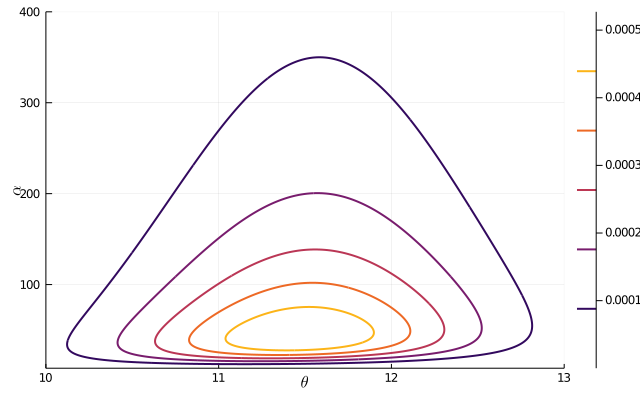
\includegraphics[width=8.5cm, height=6.5cm]{Images/TITLE/klp} }}%
    \subfloat[Distribuce $q\left(\theta,\alpha\vert\mu,\sigma,\gamma,\delta \right)$]{{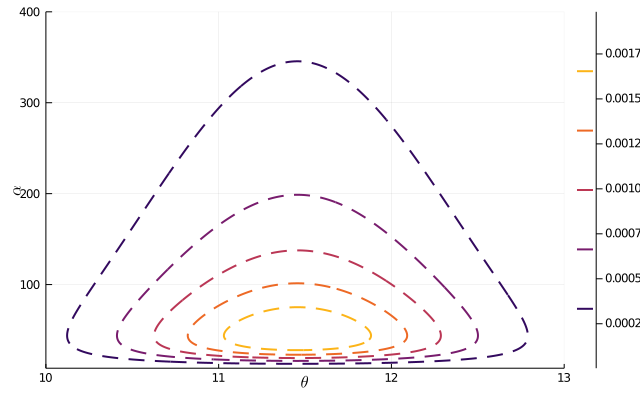
\includegraphics[width=8.5cm, height=6.5cm]{Images/TITLE/klq} }}%
    \caption{Contour plot distribucí $p(\theta,\alpha\vert y_1,y_2)$ (vlevo plnou čárou) a $q\left(\theta,\alpha\vert\mu,\sigma,\gamma,\delta \right)$ (vpravo čerchovaně), kde distribuce $q$ je vyčíslena ve vypočtených odhadech $\hat{\mu},\hat{\sigma},\hat{\gamma},\hat{\delta}$ a distribuce $p$ je vyčíslena v bodech $y_1 = 11$ a $y_2 = 12$. Je patrné, že distribuce jsou téměř totožné.  }%
    \label{kl}%
\end{figure}


\section{Teorie grafů}
Poslední teoretickou kapitolou bude vsuvka do teorie grafů. Nepůjde nám však o grafy funkcí nebo o grafy používané ve statistice. 
Tato kapitola poslouží k výhodnému popsání složitějších datových struktur.
\begin{definition}[Graf]
Grafem $G$ se rozumí dvojice $(V,H)$, kde $V$ je množina vrcholů grafu $G$ a  $H$ je množina hran tohoto grafu, přičemž jsou tyto množiny vzájemně disjunktní.
\end{definition}
Toto je zcela obecná definice grafu. Takto definovaný graf je velmi silný nástroj ke zjednodušování složitých problémů. Je vhodný pro popis takových situací, jenž můžeme znázornit pomocí konečného množství bodů, čili vrcholů $V$ a vztahů mezi nimi, které jsou znázorněny hranami $H$. 
\begin{definition}[Cesta v grafu]
Cestou v grafu rozumíme posloupnost vrcholů a hran  $(v_0, h_1, v_1,\dots ,h_t, v_t) $, kde vrcholy $v_0,\dots,v_t$ jsou navzájem různé vrcholy grafu $G$ a pro každé $i = 1,2,\dots,t$ je $e_i = \left\lbrace v_{i-1}, v_i\right\rbrace   \in H$.
\end{definition}
\begin{definition}[Orientace v grafu]
Orientovaným grafem nazveme dvojici $(V,H)$, kde $H$ je podmnožina kartézského součinu $V \times V$. Prvky $H$ pak nazýváme orientované hrany. Orientovaná hrana $h$ je tvaru $(x, y)$ a říkáme o ní, že  vychází z $x$ a končí v $y$.
\end{definition}
\begin{definition}[Souvislost grafu]
Řekneme, že graf $G$ je souvislý, jestliže pro každé dva vrcholy $v_0$ a $v_1$ existuje v $G$ cesta z $v_0$ do $v_1$.
\end{definition}
\begin{definition}[Cyklus v grafu]
Cyklem v grafu $G$ rozumíme posloupnost vrcholů a hran $(v_0, h_1, v_1,\dots ,h_t, v_t~=~v_0)$, kde vrcholy $v_0,\dots,v_{t-1}$ jsou navzájem různé vrcholy grafu $G$a pro každé $i = 1,2,\dots,t$ je $e_i = \left\lbrace v_{i-1}, v_i\right\rbrace   \in~H$.
\end{definition}
\begin{definition}[Strom]
Strom je souvislý graf neobsahující cyklus.
\end{definition}
Primárním cílem je výhodně zadefinovat stromovou strukturu, budeme totiž pracovat s orientovanými stromy, ten můžeme vidět na obrázku \ref{stromfig}. Jak na tyto definice napasovat generativní model bude hlavním cílem třetí kapitoly \ref{kapitola3}. Nejprve je nutno již zmíněný generativní model zadefinovat. 
\begin{figure}[h]
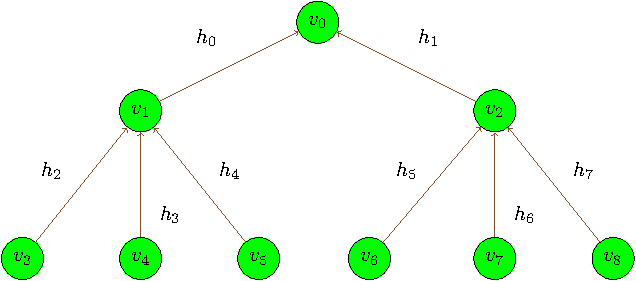
\includegraphics[width=14cm]{Images/TITLE/stromgenerally}
\centering
\caption{Příklad orientovaného stromu. Z definice stromu plyne, že mezi každými dvěma vrcholy existuje pouze jedna cesta a navíc platí, že počet vrcholů je o $1$ větší, než počet hran.}\label{stromfig}
\end{figure}








\begin{comment}
\newpage  

Pokusme se nyní využít KL - divergenci v poněkud složitějším případě. Nalezněme koeficienty polynomu pátého stupně, který nejlépe proloží dva body.\\ Uvažujme následující pravděpodobnostní model
\begin{equation*}
 P(\textbf{y},\theta \vert X,\alpha) = P(\textbf{y}\vert \theta ,X)P(\theta \vert \alpha)P(\alpha) = \pazocal{N}(X\theta, I)\pazocal{N}(0,\alpha^{-1}I)\Gamma(0,0)
 \end{equation*}
 
Dále k hledání minima využijme KL divergenci  a aproximační distribuce
\begin{equation*}
\begin{split}
q(\theta) = \pazocal{N}(\hat{\theta} , \Sigma) &\\
q(\alpha) = \Gamma(\gamma,\delta)&
\end{split}
\end{equation*}
KL divergence je tedy tvaru
\begin{equation*}
\begin{split}
KL(q\Vert p) & =  \int q(\theta)q(\alpha)\ln{\frac{q(\theta)q(\alpha)}{P(\textbf{y}\vert \theta ,X)P(\theta \vert \alpha)P(\alpha)}}\dd \alpha \dd \theta \\ &
= \int q(\theta)q(\alpha)\left(\ln{q(\theta)} + \ln{q(\alpha)} - \ln{P(\textbf{y}\vert \theta ,X)} - \ln{P(\theta \vert \alpha)} - \ln{P(\alpha)}\right) \dd \alpha \dd \theta \\&
\end{split}
\end{equation*}
Následující členy jsou opět záporně vzaté entropie jednotlivých distribucí, víme tedy že:
\begin{equation*}
\begin{split}
& \int q(\theta)\ln{q(\theta)}~\dd \theta \propto - \frac{1}{2}\ln{|\Sigma|} \\
& \int q(\alpha)\ln{q(\alpha)}~\dd \alpha = - \gamma - \ln{\delta} + \Gamma (\gamma) + (1-\gamma)\psi (\gamma)  
\end{split}
\end{equation*}
Ostatní členy budeme nyní řešit zároveň: 

\begin{equation*}
\begin{split}
\bigstar & =  \int q(\theta)q(\alpha)\left( - \ln{P(\textbf{y}\vert \theta ,X)} - \ln{P(\theta \vert \alpha)} - \ln{P(\alpha)}\right) \dd \alpha \dd \theta \\
& = \left\langle  \frac{1}{2}\left( \left(\textbf{y} -X\theta\right)\tran \left(\textbf{y} -X\theta\right) +\alpha\theta\tran\theta - 5\ln{\alpha}\right)- \ln{\alpha}\right\rangle \\
& = \left\langle \frac{1}{2} \left( \textbf{y}\tran\textbf{y} - \theta\tran X\tran\textbf{y} -\textbf{y}\tran X \theta + \theta\tran X\tran X\theta + \alpha\theta\tran\theta - 7\ln{\alpha}     \right)     \right\rangle \\
& = \left\langle \frac{1}{2}\left( \textbf{y}\tran\textbf{y} - \theta\tran X\tran\textbf{y} -\textbf{y}\tran X \theta + \tr\left(\theta\tran X\tran X\theta + \alpha\theta\tran\theta \right) - 7\ln{\alpha}     \right) \right\rangle \\
& = \left\langle \frac{1}{2}\left( \textbf{y}\tran\textbf{y} - \theta\tran X\tran\textbf{y} -\textbf{y}\tran X \theta + \tr\left( X\tran X\theta\theta\tran + \alpha\theta\theta\tran \right) -7\ln{\alpha}     \right) \right\rangle \\
& = \left\langle \frac{1}{2}\left( \textbf{y}\tran\textbf{y} - \theta\tran X\tran\textbf{y} -\textbf{y}\tran X \theta + \tr \left( \left( X\tran X + \alpha I\right) \theta\theta\tran \right) - 7\ln{\alpha}     \right) \right\rangle 
\end{split}
\end{equation*}
Po výpočtu středních hodnot dostaneme konečný výsledek, který je tvaru:
\begin{equation*}
\bigstar = \frac{1}{2}\left( \textbf{y}\tran\textbf{y} - \hat{\theta}\tran X\tran\textbf{y} -\textbf{y}\tran X \hat{\theta} + \tr \left( \left( X\tran X + \frac{\gamma}{\delta} I\right) \left(\hat{\theta}\hat{\theta}\tran + \Sigma\right)\right)  -7\left(\psi(\gamma) - \ln{\delta} \right)\right) 
\end{equation*}
Tímto máme vypočteny všechny výrazy pro optimalizaci pomocí gradientní metody.


\end{comment}


\chapter{Generativní modely}\label{generative}
 \section{Generativní model}
Ve strojovém učení se setkáváme s dvěma hlavními typy modelů a to jsou generativní modely a diskriminativní modely. Každý z nich přistupuje k zadanému problému trochu jinak. Jak už napovídá název této práce, budeme se zde zabývat výhradně generativními modely.
\begin{definition}{(Generativní model)}
Mějme nějakou množinu datových záznamů $\textbf{x} = \left(x_1,\dots,x_n \right)$, představující nezávislé proměnné a nějakou množinu $\textbf{y}$, jakožto závislé proměnné. Generativní model je potom takový model, který se učí sdruženou distribuci $p(x,y)$. Jsme tedy schopni generovat nová data pomocí původních. 
\end{definition}

\subsubsection*{Příklad}
Připomeňme nejprve, že platí $p(x,y) = p(y,x)$. V tomto okamžiku pro nás bude výhodnější hledat distribuci $p(y,x)$. Jeden ze způsobů jak odhadnout tuto distribuci, je využití součinového pravidla \eqref{chainrule}. Pomocí něj získáme tvar
\begin{equation}
p(y,x) = p(y\vert x)\cdot p(x).
\end{equation}
Problém je tedy převeden na hledání distribucí $p(y\vert x)$ a $p(x)$. Pro ilustraci uvažujme množinu datových záznamů $\textbf{x} = \left( x_1, \dots, x_n\right)$ zobrazenou na obrázku \ref{uniform}.\\
\begin{figure}[h]
\centering
\subfloat[Data, pro která hledáme distribuci $p(x,y)$.]{{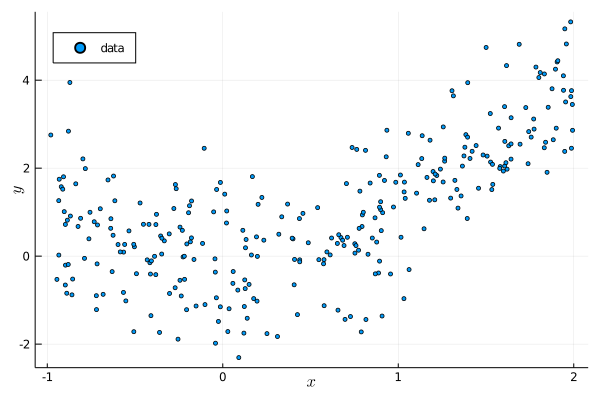
\includegraphics[width=8.4cm]{Images/TITLE/uniform} }}%
    \subfloat[Normalizovaný histogram vzorků z distribuce $p(x)$.]{{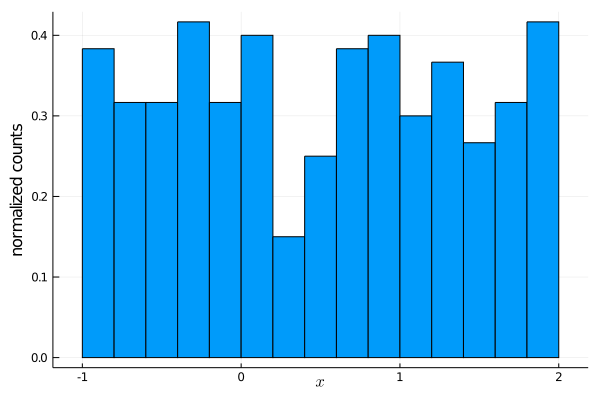
\includegraphics[width=8.4cm]{Images/TITLE/hist} }}%
    \caption{Data, pro která hledáme sdruženou distribuci $p(x,y)$ s histogramem distribuce $p(x)$. Z obrázku $(a)$ je patrné, že distribuce $p(x)$ je rovnoměrná, datové záznamy se na ose x totiž nikde neshlukují.}%
    \label{uniform}%
\end{figure}
Určit distribuci $p(x)$ není nic těžkého, můžeme ji určit například z histogramu x-ových souřadnic jednotlivých bodů nebo použít maximálně věrohodný odhad MLE [1]\\ $\textit{(Maximum Likelihood Estimation)}$. \\
 Data jsou na ose x, přesněji na intervalu $\left(a , b \right)$, rozděleny rovnoměrně. To tedy indikuje rovnoměrné rozdělení
\begin{equation}
p(x) = \mathrm{U}(a,b).
\end{equation}
Nyní přejdeme k hledání distribuce $p\left(y\vert x \right)$. Tu můžeme určit pomocí metody nejmenších čtverců \eqref{univariate__distribution_linear regression}, protože víme že pro takovou distribuci platí
\begin{equation}
 p(y\vert x) = \pazocal{N}\left(X\cdot\hat{\theta}, \sigma^2 \right),
\end{equation}
kde $X = \left(1 , x , x^2\right)$, jelikož předpokládáme, že se jedná o kvadratickou závislost a $\hat{\theta} = (\mathbb{X}\tran \mathbb{X})^{-1}\mathbb{X}\tran \textbf{y}$. Nyní máme obě složky k určení $p(y,x)$ a jsme tudíž schopni generovat nová data, protože jsme se za pomoci původních dat naučili distribuci, ze kterých jsou generována. Na obrázku \ref{generative_example} vidíme contour plot distribuce $p(y,x)$, který nám dává představu, jak tato distribuce vypadá.
\begin{figure}[h]
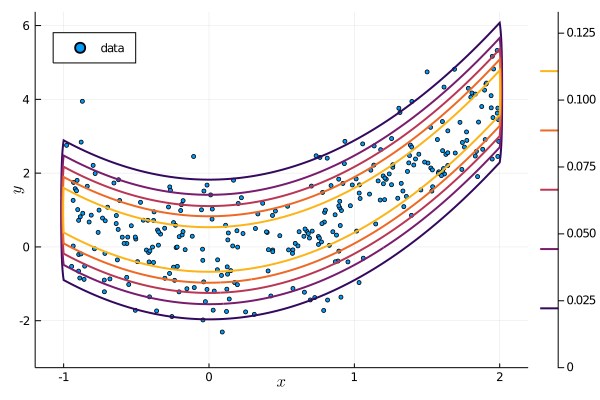
\includegraphics[width=16cm]{Images/TITLE/uniform_distribution}
\centering
\caption{Data z obrázku \ref{uniform}, tentokrát vyobrazená s contour plotem distribuce $p(y,x)$, kde $\sigma^2 = 1$, $a = -1$, $b = 2$ a $y$ závisí na $x$ kvadraticky. Distribuce je na krajích useknutá kvůli uniformnímu rozdělení - kdyby byla distribuce $p(x)$ gaussovská, byla by distribuce na okrajích zakulacená.}\label{generative_example}
\end{figure}
\section{Neuronová síť} \label{neuron}
Nejjednodušší model je takový, který obsahuje pouze lineární kombinaci vstupních proměnných $\left(x_1,\dots,x_n\right)$, tedy lineární model
\begin{equation}\label{linear_combination}
y(\textbf{x}, \textbf{w}) = w_0 + w_1x_1 + w_2x_2 + \dots + w_nx_n = w_0 + \sum_{i = 1}^{n - 1} {w_{i}x_i}.
\end{equation}
Nyní se pokusíme tento model rozšířit tím, že do něj vneseme nelineární funkce vstupních proměnných a celé to obalíme do nelineární aktivační funkce $f$, čímž získáme novou funkci
\begin{equation}\label{non-linear_combination}
y(\textbf{x}, \textbf{w}) =f\left( w_0 + \sum_{j = 1}^{m} w_{j}\phi_j\left(\textbf{x}\right)\right).
\end{equation}
Funkce $\phi_j\left(\textbf{x}\right)$ nazýváme bázové funkce. Parametr $w_0$ nám dovoluje nastavit offset, nebo-li tzv. práh $\textit{(bias)}$  v daných datech. Nyní představíme koncept neuronové sítě, který může být popsán sérií funkčních transformací. Nejprve zkonstruujeme $m$ lineárních kombinací vstupních proměnných $\left(x_1,\dots,x_n\right)$ ve tvaru
\begin{equation}
a_j = \sum_{i=1}^n w_{ji}^{(1)}x_i+w_{j0}^{(1)},
\end{equation}
kde $j$ nabývá hodnot z $\left\lbrace 1,\dots,m\right\rbrace $ a horní index $(1)$ značí, že příslušné parametry jsou v první vrstvě. Parametry $w_{ji}^{(1)}$ budeme nazývat váhy \textit{(weights)} a $w_{j0}^{(1)}$ jsou složky již zmiňovaného práhu. 
Objekty $a_j$ budeme nazývat aktivace $\textit{(activation)}$, každou aktivaci transformujeme pomocí diferencovatelné, nelinerní aktivační funkce $h$ a dostaneme
\begin{equation}
z_j = h\left(a_j\right).
\end{equation}
Z předchozí textu jasně plyne, že tento objekt odpovídá tomu v \eqref{non-linear_combination}. V kontextu neuronových sítí budeme tyto objekty nazývat skryté jednotky $\textit{(hidden units)}$, proto tedy to intuitivní značení. Nyní budeme pokračovat ve stejném postupu, vezmeme hodnoty $z_j$, opět je lineárně zkombinujeme a získáme
\begin{equation}
a_k = \sum_{j=1}^m w_{kj}^{(2)}z_j+w_{k0}^{(2)},
\end{equation}
kde $k$ nabývá hodnot z $\left\lbrace 1,\dots,l\right\rbrace$, zároveň $l$ značí celkový počet výstupů a podobně jako předtím, horní index $(2)$ značí, že příslušné parametry jsou ve druhé vrstvě. Aktivace rovněž jako v předchozím kroku obalíme do další aktivační funkce $f$ a získáme finální výstup
\begin{equation}
y_k = f\left(a_k\right).
\end{equation}
Aktivační funkci jsme označili $f$ místo $h$, poněvadž už dané jednotky nejsou skryté, ale jedná se v našem případě o výstup.\\
 Teď se ovšem pokusme pojem aktivační funkce trochu více specifikovat. Volba aktivační funkce je různá případ od případu a záleží čistě na datech, na předpokládaném tvaru distribuce výstupních dat, atd. 
Existuje jich tedy mnoho, pro ilustraci předvedeme několik nejběžnějších
\begin{equation}
\begin{split}
\textrm{Identita:}\qquad f(x) &= x , \\
\textrm{Sigmoidální:}\qquad f(x) &= \sigma\left(x\right)= \frac{1}{1 + \exp\left(-x \right)},\\
\textrm{Jednotkový skok:}\qquad f(x) &= 
 \begin{cases}
      1 & \text{pro}\ x \geq 0 \\
      0 & \text{pro}\ x < 0 
    \end{cases},
\\
\textrm{ReLU:}\qquad f(x) &= 
 \begin{cases}
      x & \text{pro}\ x \geq 0 \\
      0 & \text{pro}\ x < 0
    \end{cases} .
\end{split}
\end{equation}\\
\begin{figure}[h]
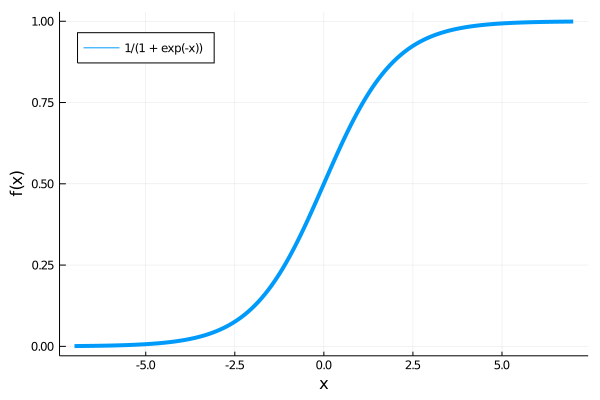
\includegraphics[width=14cm]{Images/TITLE/siigmoid}
\centering
\caption{Sigmoidální aktivační funkce. Tato funkce zajistí, aby se výstup neuronové sítě nacházel v intervalu $\left(0,1\right)$.}\label{sigmoida}
\end{figure}
Pokud tedy spojíme všechny tyto kroky a zvolíme-li například sigmoidální tvar aktivační funkce $\sigma$, dostaneme tvar dvouvrstvé neuronové sítě 
\begin{equation}
y_k\left(\textbf{x},\textbf{w}\right) = \sigma\left(\sum_{j=1}^m w_{kj}^{(2)}h\left(\sum_{i=1}^n w_{ji}^{(1)}x_i+w_{j0}^{(1)}\right)+w_{k0}^{(2)}\right) .
\end{equation}
Všechny váhy a složky prahu byly umístěny do vektoru vah $\textbf{w}$. Neuronová síť je jednoduše řečeno pouze nelineární funkce z množiny vstupních proměnných $\left\lbrace x_i\right\rbrace_{i = 1}^n $ do množiny $\left\lbrace y_k\right\rbrace_{k = 1}^l $, určená vektorem $\textbf{w}$.   Na množství vrstev v neuronové síti se meze nekladou, alternativně lze sestrojovat další a další vrstvy. 
\section{Variační autoencoder}
Jedna z mnoha metod, jak využít neuronové sítě, je metoda variačního autoencoderu. Cílem  je najít hustotu $p(\textbf{x})$ vzorků $\left\lbrace x_{i} \right\rbrace^n_{i=1} $.
Předpokládáme následující vztahy
\begin{equation}
\textbf{x} = f_{\theta}(\textbf{z}) + \epsilon ,
\end{equation}
kde $\epsilon \sim \pazocal{N}\left(0,\sigma^2\cdot\mathbb{I}   \right)$ a $f_{\theta}(\textbf{z})$ je neuronová síť.  Využijeme následující formu aproximace
\begin{equation}
p(\textbf{x}) = \int p(\textbf{x}\vert \textbf{z})p(\textbf{z})\dd \textbf{z} .
\end{equation}
Podle vztahu pro $\textbf{x}$ určíme distribuci $p\left(\textbf{x}\vert \textbf{z}\right)$ a $p\left(\textbf{z}\right)$ zvolíme jednoduše
\begin{equation}
\begin{split}
 p(\textbf{x}\vert \textbf{z}) &= \pazocal{N}\left(f_{\theta}(\textbf{z}),\sigma^2\cdot\mathbb{I} \right) \\
p(\textbf{z}) &= \pazocal{N}\left(0,\mathbb{I} \right)
\end{split}
\end{equation}

\subsection{Naivní přístup}
K nalezení $p(\textbf{x})$ je třeba najít parametry $\theta$ transformace $f_{\theta}(\textbf{z})$, proto zkusme sestavit věrohodnostní funkci $ \log p\left( \textbf{x}\right) = \log \prod_{i = 1}^n p\left(x_i \right) $  a minimalizovat 
\begin{equation}
\begin{split}
\hat{\theta} & = \argmin_{\theta} \sum_{i=1}^n \log p\left(x_{i} \right)\\
& =  \argmin_{\theta} \sum_{i=1}^n \log \int \pazocal{N}\left(f_{\theta}(z_j),\sigma^2 \right)\pazocal{N}\left(0,1 \right)    \dd z_j \\
& = \argmin_{\theta} \sum_{i=1}^n \ \log\sum_{j=1}^n \exp \left\lbrace -\frac{1}{2\sigma^2} \left(x_i - f_{\theta}(z_j)  \right)^2 \right\rbrace \cdot \exp \left\lbrace -\frac{z_j^2}{2} \right\rbrace .
\end{split}
\end{equation}
Integrace přes $\textbf{z}$ je nahrazena vzorkováním. Tento postup ovšem při minimalizaci nemusí konvergovat ke správným výsledkům.
\subsection{Variační Bayseova metoda}
Lepší metodou se ukazuje vzorkovat z podmíněné distribuce $q(\textbf{z}\vert \textbf{x})$ a využít ELBO

\begin{equation}
\begin{split}
D_{KL}\left(q\left(\textbf{z}\vert \textbf{x} \right) \Vert p(\textbf{z}\vert \textbf{x})\right) & = 
 \mathbb{E}_q\left[\log q(\textbf{z}\vert \textbf{x}) - \log p\left(\textbf{z}\vert \textbf{x} \right)\right] \\
 & =  \mathbb{E}_q\left[\log q(\textbf{z}\vert \textbf{x}) - \log p(\textbf{x}\vert \textbf{z}) - \log p(\textbf{z}) + \log p(\textbf{x})   \right] .
 \end{split}
\end{equation}
Tuto rovnici můžeme přepsat pomocí KL-divergence 
\begin{equation}
\log p(\textbf{x}) - D_{KL}\left(q\left(\textbf{z}\vert \textbf{x} \right) \Vert p(\textbf{z}\vert \textbf{x})\right) = \mathbb{E}_q\left[\log p(\textbf{x}\vert \textbf{z}) \right] - D_{KL}\left(q\left(\textbf{z}\vert\textbf{x} \right) \Vert p(\textbf{z})\right) ,
\end{equation}
kde pravá strana této rovnice je lower bound objektu $\log p(\textbf{x})$.
Jestliže vybereme parametrickou formu distribuce
\begin{equation}
q\left(\textbf{z}\vert \textbf{x} \right) = \pazocal{N}\left(\mu_{\phi}(\textbf{x}), \diag\left(\sigma^2_{\phi}(\textbf{x})\right) \right) ,
\end{equation}
můžeme parametry $\theta$ a $\phi$ minimalizovat zároveň a to následovně
\begin{equation}
\begin{split}
\hat{\theta},\hat{\phi} & = \argmin_{\theta, \phi}\sum_{i=1}^n\log p\left(x_i\right) \\
& = \argmin_{\theta, \phi}\left\lbrace  \mathbb{E}_q\left[\log p(\textbf{x}\vert \textbf{z}) \right] - D_{KL}\left(q\left(\textbf{z}\vert \textbf{x} \right) \Vert p(\textbf{z})\right)\right\rbrace . 
\end{split}
\end{equation}
V metodě variačního autoencoderu jsou nezbytné následující dva fakty. První je trik v reparametrizaci
\begin{equation}
\textbf{z} = \mu_{\phi}(\textbf{x}) + \diag\left(\sigma^2_{\phi}(\textbf{x})\right)^{1/2}\odot\epsilon ,
\end{equation}
kde $\odot$ značí Hadamardův součin, čili součin po složkách.
To můžeme zapsat jednodušeji takto
\begin{equation}
z_i = \mu_{\phi}(x_i) + \sigma_{\phi}(x_i)\cdot\epsilon_i .
\end{equation}
Nejedná se v podstatě o nic jiného, než o transformaci náhodné veličiny.
Druhou důležitou věcí je fakt, že KL-divergence dvou gaussovských distribucí má analytické řešení
\begin{equation}
\begin{split}
 D_{KL}\left(q\left(\textbf{z}\vert \textbf{x} \right) \Vert p(\textbf{z})\right) & = \frac{1}{2}\left[\tr\left(\diag\left(\sigma_{\phi}^2(\textbf{x})\right)\right) - \mu_{\phi}\tran(\textbf{x})\mu_{\phi}(\textbf{x}) - k - \log\det \diag\left(\sigma_{\phi}^2(\textbf{x})   \right)\right] \\
 & = \frac{1}{2}\left[\sum_{l = 1}^k(\sigma_{\phi}^2(\textbf{x})) -\mu\tran(\textbf{x})\mu_{\phi}(x) - k - \sum_{l = 1}^k\log\sigma_{\phi}^2(\textbf{x})    \right] .
\end{split}
\end{equation}
Kdybychom totiž nevybrali aproximační distribuci gaussovskou, nemohli bychom tímto způsobem $\hat{\theta},\hat{\phi}$ určit. Díky tomu získáme konečný tvar
\begin{equation}\label{řešení_VAE}
\hat{\theta},\hat{\phi} = \argmin_{\theta, \phi}\left[\sum_{i = 1}^n\sum_{j = 1}^p \left[ x_i - f_\theta \left(\mu_{\phi}(x_i) + \sigma_{\phi}(x_i)\cdot\epsilon_{i,j}  \right)        \right]^2 - \frac{1}{2}\left[\sum_{l = 1}^k(\sigma^2_{\phi}(x_i)) -\mu_{\phi}\tran(x_i)\mu_{\phi}(x_i) - k - \sum_{l = 1}^k\log\sigma^2_{\phi}(x_i)   \right] \right].
 \end{equation}
\subsection*{Příklad}
Jednoduchým příkladem může být následující problém, kde v rovnici $x = f_\theta\left(z\right) + \epsilon$,  je funkce $f$ pouze ve tvaru
\begin{equation}
 f_\theta\left(z\right) = z + \theta.
\end{equation}
V tomto případě můžeme spočítat analyticky následující distribuce
\begin{equation}
\begin{split}
p(x) &= \pazocal{N}\left(\theta, \sigma^2 + 1\right) \\
p(z\vert x) &=  \pazocal{N}\left(\frac{x - \theta}{\sigma^2 + 1}, \frac{\sigma^2}{\sigma^2 +1 } \right).
\end{split}
\end{equation}
Díky tomu můžeme zvolit následující formu aproximační distribuce 
\begin{equation}
q\left(z\vert x\right) = \pazocal{N}\left(\gamma x - \theta, \gamma \sigma^2 \right),
\end{equation} 
kde $\gamma = \frac{1}{\sigma^2 + 1}$,
čímž jsme získali $\mu_\phi\left(x\right)$ a $\sigma_\phi(x)$.  Nyní zbývá dosadit do \eqref{řešení_VAE} - tím získáme 
\begin{equation}
\hat{\theta},\hat{\phi} = \argmin_{\theta, \phi}\left[\sum_{i = 1}^n\sum_{j = 1}^p \left[ x_i - f_\theta \left(\mu_{\phi}(x_i) + \sigma_{\phi}(x_i)\cdot\epsilon_{i,j}  \right)        \right]^2 - \frac{1}{2}\left[\sum_{l = 1}^k(\sigma^2_{\phi}(x_i)) -\mu_{\phi}\tran(x_i)\mu_{\phi}(x_i) - k - \sum_{l = 1}^k\log\sigma^2_{\phi}(x_i)   \right] \right]
 \end{equation}
$  $\chapter{Stromové struktury}\label{kapitola3}
Stromovou strukturou dat rozumíme množinu datových záznamů popsaných pomocí množiny vrcholů a hran. Vrcholy dané stromové struktury představují jednotlivé body $x$ a $y$. V podstatě si to můžeme představit opravdu jako strom - má jeden kořen, v první úrovni se dělí na $k_1$ větví, každá další větev se v druhé úrovni dělí na $k_{2_i}$ a tak dále.  My se v této práci budeme zabývat pouze kořenem a první úrovní větví. Ilustrujeme to na jednoduchém příkladu.
\subsection*{Příklad}
Mějme vektor pozorování $\textbf{y} = \left(y_1,\dots,y_n \right)$. Předpokládejme takový model, který ke každému $y_i \in \textbf{y}$, přiřazuje vektor datových záznamů $\textbf{x}_{i}$, $i \in \left\lbrace 1,\dots,n \right\rbrace$, přičemž každý $\textbf{x}_i $ má různý počet prvků $x_j^{(i)}$, $j\in\left\lbrace 1,\dots,k_i \right\rbrace$. Máme tedy $\pazocal{X} = \left(\textbf{x}_1,\dots,\textbf{x}_n \right)$, kde každý vektor $\textbf{x}_i$ může mít jiný počet prvků $k_i$. Celkový počet datových záznamů v $\pazocal{X}$ je $m$, platí tedy $\sum_{i = 1}^{n}\sum_{j = 1}^{k_i} x_j^{(i)} = m$.  Přiřazení probíhá následujícím způsobem
\begin{equation}
\begin{split}
\textbf{x}_1 & \longmapsto  y_1, \\
\textbf{x}_2 & \longmapsto  y_2,\\
\vdots \\
\textbf{x}_n & \longmapsto   y_n.
\end{split}
\end{equation}
Jednoduše řečeno je to přiřazení popořadě. Názorně to můžeme vidět na obrázku \ref{bag}.



\begin{figure}[h]
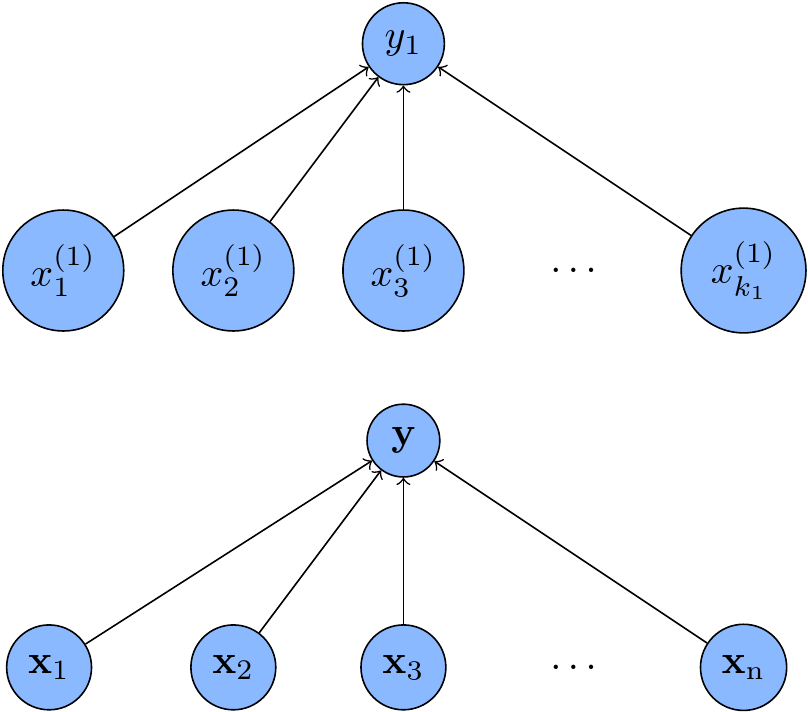
\includegraphics[width=9cm]{Images/TITLE/strom}
\centering
\caption{Grafické znázornění přiřazení jednotlivých $x_j^{(i)}$ k $y_i$ v horní části, vektorové přiřazení v dolní části obrázku.}\label{bag}
\end{figure}

Vektor takových $x_j^{(i)} \in \textbf{x}_i$ , přiřazených k jednomu $y_i$ nazveme plukem $\textit{(bag)}$. Abychom to uvedli do kontextu stromových struktur, znamená to  že $y_i$ jsou uzly jednoho typu, $x_j^{(i)}$ jsou uzly druhého typu, mezi nimiž existují hrany. \\
Počet prvků v jednom pluku $k_i$ nechť je generován například Poissonovým rozdělením, tedy
\begin{equation}
p\left(k_i\right) = \mathrm{Po}\left(\lambda\right) \quad \forall i \in \left\lbrace1,\dots,n\right\rbrace.
\end{equation}
Potom všechny prvky $\pazocal{X}$ nechť jsou například generovány pomocí uniformního rozdělení
\begin{equation}
p\left(x_j^{(i)}\right) = \mathrm{U}\left(a,b\right) \quad \forall i \in \left\lbrace1,\dots,n\right\rbrace\quad \&\quad \forall j \in \left\lbrace1,\dots,k_i\right\rbrace.
\end{equation}
 Jednotlivá $y_i$ potom můžou být určena nějakou závislostí na $\textbf{agregační funkci}$ prvků v plucích k  nim přiřazených. $\textbf{Agregační funkcí}$ budeme rozumět takovou funkci, která dokáže seskupit, nebo-li agregovat, vícero datových záznamů do jednoho. Nejčastěji používané agregační funkce jsou aritmetický průměr, maximum, minimum, nebo součet.    \\
 Pokusme se nalézt sdruženou distribuci $p(y, \bar{x}_{i})$, kde  $\bar{x}_{i}$ značí aritmetický průměr prvků v i-tém pluku, čili
  \begin{equation}
  \bar{x}_{i} = \frac{1}{k_i}\sum_{l = 1}^{k_i} x_l^{(i)}. 
 \end{equation}
Použijeme opět součinové pravidlo 
\begin{equation}
p(y, \bar{x}_{i}) = p(y\vert \bar{x}_{i})\cdot p(\bar{x}_{i})
\end{equation}
a pokusíme se nalézt tyto dvě distribuce. Tento postup je nám známý už z kapitoly \eqref{generative}. Pro určení podmíněné distribuce $p(y, \bar{x}_{i})$ použijeme opět metodu nejmenších čtverců a dostaneme 
\begin{equation}
p(y, \bar{x}_{i}) = \pazocal{N}\left(X\cdot\hat{\theta}, \sigma^2  \right).
\end{equation}
Ovšem zde jsou prvky vektoru $X$ právě aritmetické průměry, tedy
\begin{equation}
X = \left( 1 , \bar{x}, \bar{x}^2, \dots, \bar{x}^p\right).
\end{equation}
Určit distribuci $p(\bar{x}_{i})$ lze určit obdobně pomocí histogramu. Navíc víme-li, že se jedná o výběrové průměry, je z centrální limitní věty [] jasné, že se bude jednat o normální rozdělení. Střední hodnotu můžeme odhadnout výběrovým průměrem z $\bar{x}_{i}$, tedy
\begin{equation}
 \bar{\bar{x}} = \frac{1}{n}\sum_{i = 1}^n \bar{x}_{i}
\end{equation}
  a rozptyl odhadneme pomocí výběrového rozptylu 
  \begin{equation}
  \Var\left(\bar{x}_{i}\right) = \frac{1}{n}\sum_{i = 1}^n \left( \bar{x}_{i} - \bar{\bar{x}}\right)^2.
\end{equation}  
 Oba objekty jsou maximálně věrohodnými odhady Gaussova rozdělení.
Získáme tak tvar
\begin{equation}
p(\bar{x}_{i}) = \pazocal{N}\left(\bar{\bar{x}}_{i},\Var\left(\bar{x}_{i}\right) \right).
\end{equation}
Tímto máme spočtené obě složky. Pro vizualizaci sdružené distribuce $p(y, \bar{x}_{i})$ využijeme opět contour plot. Jak tato distribuce vypadá vidíme na obrázku \ref{stromy_done}. \\
\begin{figure}[h]
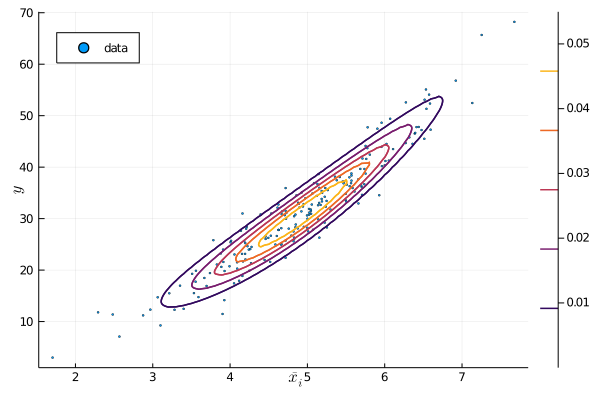
\includegraphics[width=14cm]{Images/TITLE/strom_done}
\centering
\caption{Countour plot distribuce $p(y, \bar{x}_{i})$, kde $m = 200, \lambda = 10, a = 0, b = 10$ a $y$ závisí na $\bar{x}_{i}$ kvadraticky.}\label{stromy_done}
\end{figure}
Najít distribuci $p(y\vert x)$ není v tomto případě snadný úkol, proto jsme se omezili pouze na hledání distribuce z průměrů jednotlivých složek $\pazocal{X}$.



\subsection*{Příklad}
Dalším příkladem stromové struktury může být následující zjednodušený finanční model, který udává velikosti transakcí na bankovním účtu klientů. Budou to dvě gaussovské směsi 
\begin{equation}
\begin{split}
p(x\vert y = 1) & = w_1\cdot\pazocal{N}\left(\mu_1,\sigma^2_1\right) + (1 - w_1)\cdot\pazocal{N}\left(\mu_2,\sigma^2_2 \right),\\
p(x\vert y = 0) & = w_2\cdot\pazocal{N}\left(\mu_3,\sigma^2_3\right) + (1 - w_2)\cdot\pazocal{N}\left(\mu_4,\sigma^2_4 \right)
\end{split}
\end{equation}
 a z každé z nich máme $n$ vzorků, navíc $y$ je teď diskrétní náhodná veličina nabývajících pouze dvou hodnot z $\left\lbrace 0,1 \right\rbrace$ a $w \in \left[0,1\right]$ je váha.  Veličina $y$ udává, zda je klient schopen splácet půjčku, kde $0$ znamená $\textit{ne}$  a $1$ znamená $\textit{ano}$.
 Dále budeme uvažovat počty transakcí $N_x$ daného klienta a distribuce
\begin{equation}
 \begin{split}
p(N_x\vert y = 1) & = \mathrm{Po}\left(\lambda_1 \right), \\
p(N_x\vert y = 0) & = \mathrm{Po}\left(\lambda_2 \right),
\end{split}
 \end{equation}
 což tedy udává takovou distribuci počtů transakcí klienta, jestli je schopen nebo není schopen splácet půjčku. \\
 Jak takové distribuce odhadnout? Jelikož známe tvar těchto distribucí, můžeme použít maximálně věrohodný odhad MLE. Sestavíme věrohodnostní funkce
\begin{equation}
\ell\left(\mu_1,\mu_2,\sigma_1^2, \sigma_2^2 \right) = \log \left( \prod_{i = 1}^n p(x_i \vert y = 1) \right)   
\end{equation}
jednotlivých distribucí. Alternativně pro ostatní distribuce, pro které potřebuje odhadnout parametry.  Věrohodnostní funkci opět numericky maximalizujeme pomocí optimalizační metody ADAM a získáme
 \begin{equation}
\hat{\mu_1}, \hat{\mu_2},\hat{\sigma_1^2},\hat{\sigma_2^2} =  \argmax_{\mu_1,\mu_2,\sigma_1^2, \sigma_2^2}  \log \left( \prod_{i = 1}^n p(x_i \vert y = 1) \right).   
 \end{equation}
Pro Poissonovo rozdělení existuje však analytické řešení 
\begin{equation}
\hat{\lambda} = \frac{1}{n}\sum_{j = 1}^{n}x_j .
\end{equation}
Nutno podotknout, že složitější gaussovskou směs bychom pomocí MLE odhadovat nemohli. Pro odhad parametrů gaussovské směsi se běžně používá tzv. EM algoritmus $\textit{(Expectation Maximization)}$ \cite{bishop}, který je iterativní a navíc využívá latentních proměnných. K odhadu tedy potřebujeme nějakou dodatečnou informaci, typicky informaci o tom, do kterého shluku $\mathit{(clusteru)}$ daný bod patří. Nicméně, že zde funguje i MLE se můžeme přesvědčit na obrázku \ref{ggm}.
 \begin{figure}[h]
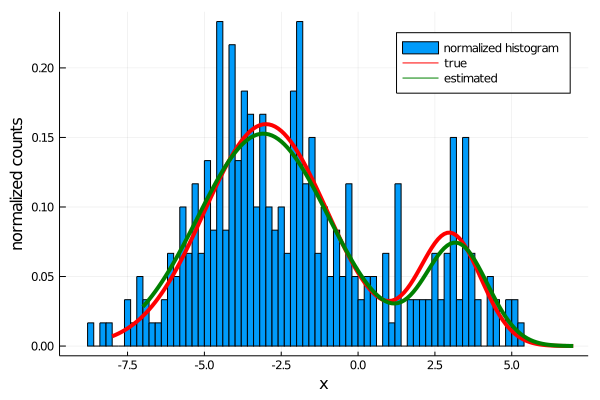
\includegraphics[width=14cm]{Images/TITLE/ggmdone}
\centering
\caption{Distribuce $p(x\vert y = 1) = 0,8\cdot\pazocal{N}\left(-3,2\right) + 0,2\cdot\pazocal{N}\left(3,1 \right)$ (červeně) a histogram vzorků z této distribuce. Dále odhad této distribuce (zeleně) pomocí MLE odhadu parametrů. Získali jsme $\hat{p}(x\vert y = 1) = 0,82\cdot\pazocal{N}\left(-2.96,2.01\right) + 0,18\cdot\pazocal{N}\left(2.86,1.06 \right)$.}\label{ggm}
\end{figure}
 
 
\chapter*{Závěr}

\pagestyle{plain}

\addcontentsline{toc}{chapter}{Záv\v{e}r}

Text závěru....
\begin{thebibliography}{1}
\bibitem{bishop}Christopher M. Bishop: \emph{Pattern recognition and machine learning}. New York: Springer, 2006. Information science and statistics. ISBN 0-387-31073-8.
\bibitem{mle}\emph{301 Moved Permanently} [online]. Copyright © [cit. 08.07.2020]. Dostupné z: http://statweb.stanford.edu/~susan/courses/s200/lectures/lect11.pdf

\end{thebibliography}

\end{document}
